% RASCUNHO. Resultados das fases 11 a 14, no formato de ic_report.tex.
% Compilar a partir de report/artigo_kernel/:  latexmk -pdf -outdir=<pasta fora do repo> artigo_kernel.tex
% As figuras vêm direto de results/figures_generated/; os títulos embutidos são cortados com trim e a informação vai para a legenda.
% \pendente{...} marca, em vermelho, o que depende de treinos em andamento (hoje: as seeds 43 e 44 do Fire 3x3 com dois blocos por
% estágio, sec:unidades). A fase 14 (Winograd-FPGA na receita única, docs/logs/PHASE14_LOG.md) terminou em 2026-11-09; as seeds 43 e 44
% da fase 13 entraram em 2026-11-07, e a etapa de blocos Bottleneck e Fire (7 de 7) em 2026-11-13 (docs/logs/PHASE13_LOG.md).
\documentclass[conference]{IEEEtran}
\IEEEoverridecommandlockouts
\renewcommand{\figurename}{Figura}
\renewcommand{\tablename}{Tabela}
\renewcommand{\appendixname}{Apêndice}
\renewcommand{\abstractname}{Resumo}
\usepackage{cite}
\usepackage{amsmath,amssymb,amsfonts}
\usepackage{graphicx}
\usepackage{textcomp}
\usepackage{booktabs}
\usepackage{multirow}
\usepackage{xcolor}
\usepackage{placeins}

\graphicspath{{../../results/figures_generated/}}
\newcommand{\pendente}[1]{\textcolor{red}{[#1]}}
\newcommand{\by}{\ensuremath{\times}}
\newcommand{\mn}{\ensuremath{-}}

% Mesmo ajuste do ic_report.tex: a sobra vai para o pé da coluna em vez de abrir o texto.
\raggedbottom
% Deixa até três figuras de largura total por página, para o texto não ficar espalhado entre elas.
\setcounter{dbltopnumber}{3}
\renewcommand{\dbltopfraction}{0.95}
\renewcommand{\dblfloatpagefraction}{0.7}

\begin{document}

\title{Kernels Pequenos em CNNs para Aceleração Winograd: Quanto Custam e Como Recuperar a Acurácia}

\author{
\IEEEauthorblockN{Rafael Silva de Souza}
\IEEEauthorblockA{Curso de Engenharia de Computação \\
Instituto de Informática \\
Universidade Federal do Rio Grande do Sul (UFRGS) \\
rafael.souza@inf.ufrgs.br}
\and
\IEEEauthorblockN{Mateus Grellert da Silva}
\IEEEauthorblockA{Professor Adjunto, Orientador \\
Instituto de Informática \\
Universidade Federal do Rio Grande do Sul (UFRGS) \\
mateus.grellert@inf.ufrgs.br}
}

\maketitle
% IEEEtran em modo conference não numera as páginas; o estilo plain põe o número no rodapé.
\thispagestyle{plain}
\pagestyle{plain}

\begin{abstract}
O algoritmo de Winograd faz convoluções com menos multiplicações, mas só compensa com kernels pequenos, como 2\by2 e 3\by3, enquanto
redes clássicas, como a AlexNet, usam kernels bem maiores. Este artigo mede quanto custa trocar esses kernels e como recuperar a
acurácia perdida. Para isso, fizemos 287 treinos no Tiny ImageNet e no CIFAR-100, quase todos com uma única receita e mudando um fator
de cada vez, e avaliamos cada rede em FP32 e em INT8. O custo depende da rede e do classificador. Com classificador GAP e BatchNorm,
passar de 3\by3 para 2\by2 custa de 1,0 a 2,4 pontos percentuais (p.p.) na AlexNet, na VGG16 e na ResNet-18. Na AlexNet com GAP, essa
perda some quando as duas redes têm a mesma capacidade, e a rede inteira em 2\by2 fica só 0,5 p.p. abaixo dos kernels originais, com
69\% menos multiplicações; com classificador totalmente conectado, a mesma AlexNet perde 6,5 p.p. (uma seed). O stride da primeira
camada pesa mais que o kernel (mediana de $+$9,7 p.p.), duas convoluções pequenas por estágio recuperam a perda, e a quantização para
INT8 quase não muda a acurácia. Com isso, uma AlexNet só com kernels 2\by2 chega a 60,63\% em INT8, contra 59,45\% da VGG16 (médias de
3 seeds), com um sexto dos parâmetros. Por fim, simulamos a aritmética de um acelerador Winograd em FPGA em 16 redes: o F(2,3) custa
0,2 p.p. (mediana), o F(4,3) custa 6,3 p.p., e o F(6,3) derruba seis das redes profundas para perto do acaso.
\end{abstract}

\section{Introdução}

O algoritmo de Winograd faz a mesma convolução com menos multiplicações \cite{lavin2016fast}, mas é usado quase sempre com kernels
pequenos, porque a precisão numérica piora rápido com o tamanho da convolução \cite{barabasz2020error}. Redes clássicas seguem outro
caminho: a AlexNet \cite{krizhevsky2012imagenet}, por exemplo, começa com kernels 11\by11 e 5\by5. A pergunta natural é quanto se perde
ao trocar esses kernels por outros menores.

A literatura não dá uma resposta única. De um lado, a VGG mostrou que duas convoluções 3\by3 seguidas enxergam a mesma região que uma
5\by5 \cite{simonyan2015very}. De outro, trabalhos mais recentes obtêm bons resultados com kernels grandes, usando convoluções
\textit{depthwise} \cite{liu2022convnext,ding2022scaling}, um tipo de convolução que não recebe a aceleração de Winograd nas
implementações que medimos \cite{souza2026relatorio}.

Em um relatório anterior \cite{souza2026relatorio}, comparamos variantes da AlexNet que diferiam em mais de um aspecto e que treinaram
por números diferentes de épocas. Isso atrapalha a leitura dos resultados, porque o treino pode pesar mais que a própria arquitetura
\cite{bello2021revisiting,wightman2021resnet} e uma comparação justa precisa controlar o que muda \cite{radosavovic2019network}. Neste
artigo, refazemos o estudo com uma única receita de treino, mudando uma coisa de cada vez. A Seção~\ref{sec:fundamentos} explica os
conceitos usados, e a Seção~\ref{sec:metodo} descreve o método e o motivo de cada escolha. A Figura~\ref{fig:caminho} resume o caminho
da AlexNet original até a melhor rede, e os resultados respondem a dez perguntas:
\begin{enumerate}
\item De onde vem a baixa acurácia da AlexNet em imagens pequenas? (Seção~\ref{sec:geometria})
\item Quanto custa restringir o kernel? (Seção~\ref{sec:custo})
\item O 2\by2 perde pelo kernel ou pela capacidade? (Seção~\ref{sec:controles})
\item Dá para recuperar a perda sem um corpo de kernel grande? (Seção~\ref{sec:recuperar})
\item A quantização INT8 atrapalha? (Seção~\ref{sec:int8})
\item Quanto da rede cabe em um acelerador Winograd? (Seção~\ref{sec:hardware})
\item Os resultados valem em outras condições? (Seção~\ref{sec:robustez})
\item Os ganhos se somam? (Seção~\ref{sec:combinacoes})
\item Blocos Bottleneck e Fire barateiam o melhor corpo? (Seção~\ref{sec:unidades})
\item Quanto a aritmética do acelerador Winograd custa em acurácia? (Seção~\ref{sec:numerica})
\end{enumerate}

\begin{figure*}[!t]
\centering
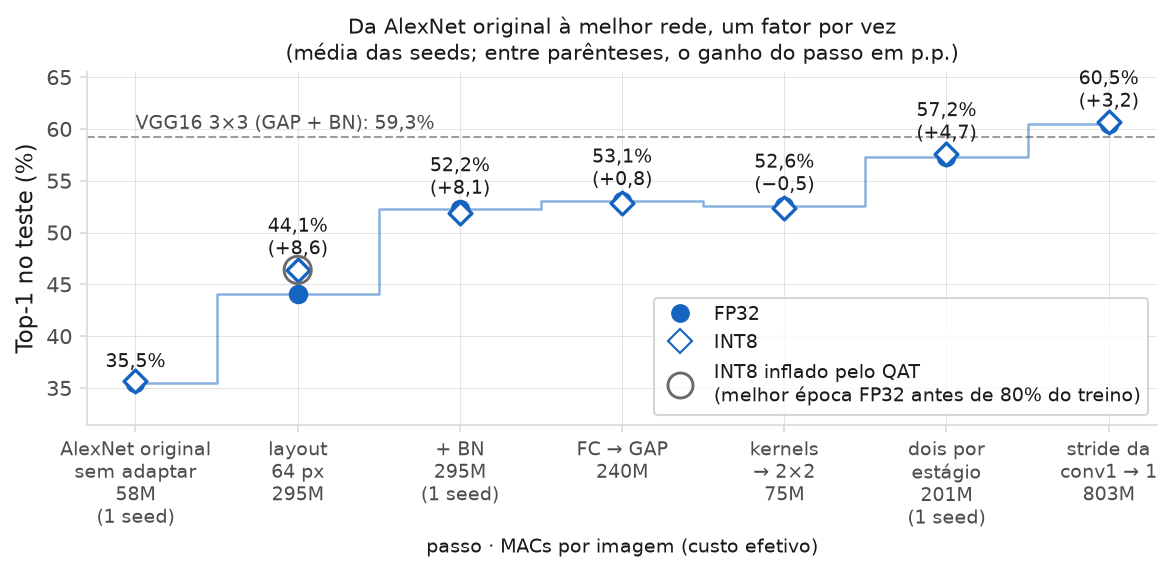
\includegraphics[width=0.86\textwidth,trim=0 0 0 32.2,clip]{phase_13_hybrids/02_caminho.png}
\caption{Da AlexNet original à melhor rede, mudando um fator por vez (top-1 no teste; média das seeds quando há mais de uma). Os dois
últimos passos têm dez convoluções; os anteriores, cinco. Em cima de cada passo, a acurácia FP32 e, entre parênteses, quanto ele ganhou.
Embaixo, os MACs em custo efetivo. Os maiores passos são o layout,
o BN, as duas convoluções por estágio e o stride 1; trocar todos os kernels por 2\by2 custa 0,5 p.p. e corta 69\% dos MACs. A linha tracejada é a
VGG16 3\by3 com GAP e BN.}
\label{fig:caminho}
\end{figure*}

Nossas principais conclusões são:
\begin{itemize}
\item O custo do kernel depende da rede e do classificador. Com GAP e BatchNorm, passar de 3\by3 para 2\by2 custa de 1,0 a 2,4 p.p. nas três famílias testadas. Com FC e Dropout, esse custo sobe na AlexNet e some na VGG16.
\item Na AlexNet com GAP e BatchNorm, o 2\by2 perde para o 3\by3 por ter menos capacidade, não por causa do kernel: com os mesmos MACs e parâmetros, os dois empatam.
\item O stride da conv1 ($+$9,7 p.p.) e o BatchNorm ($+$5,2 p.p.) pesam mais que trocar os kernels originais por 3\by3 ($-$1,5 p.p.) ou 3\by3 por 2\by2 ($-$2,5 p.p.), nas medianas de todos os pares, com e sem FC.
\item Duas convoluções pequenas por estágio recuperam a perda. Com esse corpo, o 2\by2 fica acima do 3\by3 nos 8 pares da seed 42, com cerca de metade dos MACs. Com as seeds 43 e 44, a vantagem se repete nas três seeds sem atalho e em duas de três com atalho.
\item A quantização INT8 quase não muda a acurácia, seja qual for o kernel. Os grandes ``ganhos'' em INT8 vêm de treino extra.
\item Na aritmética do acelerador Winograd, o tamanho do bloco de saída custa mais acurácia do que a troca de kernel custou no estudo principal: F(2,3) quase não custa, F(4,3) custa cerca de 6 p.p., e F(6,3) leva seis redes profundas ao acaso.
\item Boa parte dos ganhos atribuídos antes a blocos de compensação vinha das diferenças de treino.
\end{itemize}

\section{Fundamentos}
\label{sec:fundamentos}

\subsection{Convolução de Winograd}

Uma convolução comum desliza o kernel sobre o mapa de entrada e multiplica cada peso por cada valor coberto. O algoritmo de Winograd,
em vez disso, calcula um bloco inteiro da saída de uma vez: transforma um trecho da entrada e o kernel para outro domínio, multiplica
elemento a elemento e transforma o resultado de volta \cite{lavin2016fast}.

Escrevemos F($m$,$r$) para blocos de saída $m\times m$ e kernel $r\times r$. O método direto usa $m^2r^2$ multiplicações, e o de Winograd,
$(m+r-1)^2$. Assim, F(2,2) usa 9 em vez de 16 (1,78 vez menos), F(2,3) usa 16 em vez de 36 (2,25 vezes menos) e F(4,3) usa 36 em vez de 144
(4 vezes menos).

Três consequências importam neste artigo. A primeira é que o ganho tem um preço numérico: o limite do erro cresce exponencialmente com
o tamanho da convolução \cite{barabasz2020error}, e por isso se usam kernels e blocos pequenos. A segunda é que um kernel menor
economiza menos: o 2\by2 ganha menos com Winograd que o 3\by3, e o 1\by1 não ganha nada, pois a fórmula dá $m^2$ nos dois métodos. A
terceira é que nem toda convolução se beneficia. Consideramos elegíveis só as convoluções densas de stride 1, porque o stride maior
que 1 quebra os blocos de saída vizinhos e as convoluções \textit{depthwise} não recebem a aceleração nas implementações que medimos
\cite{souza2026relatorio}.

\subsection{Geometria da rede}

A AlexNet tem cinco convoluções: chamamos a primeira de \textit{conv1} e as demais de \textit{corpo}. Três escolhas definem sua
geometria: o \textit{kernel} (a região que cada convolução olha), o \textit{stride} (quantos pixels ela avança a cada passo) e os
\textit{max-pools} (que reduzem o mapa pela metade). Juntas, elas determinam o \textit{mapa final}, a grade de valores que chega ao
classificador. Já o \textit{campo receptivo} é a região da imagem que influencia uma unidade da rede; duas convoluções 3\by3 seguidas,
por exemplo, têm o campo receptivo de uma 5\by5, com menos pesos \cite{simonyan2015very}.

\subsection{Classificador e regularização}

O \textit{classificador} é a parte final da rede, e usamos dois tipos. No \textit{GAP}, tiramos a média de cada canal do mapa final e
usamos uma única camada linear. No \textit{FC}, que tem muito mais parâmetros, o mapa é redimensionado para 6\by6 (na VGG16, 7\by7) e
passa por três camadas totalmente conectadas, como na AlexNet e na VGG originais. Duas técnicas de regularização aparecem ao longo do
texto: o \textit{BatchNorm} (BN), que normaliza as ativações de cada camada, e o \textit{Dropout}, que desliga metade das unidades, ao
acaso, durante o treino.

\subsection{Quantização}

Em \textit{FP32}, a rede usa números de ponto flutuante de 32 bits; em \textit{INT8}, inteiros de 8 bits, que ocupam um quarto da
memória e são mais baratos em hardware. O \textit{Quantization-Aware Training} (QAT) é um treino que simula os arredondamentos do INT8,
para que a rede se ajuste a eles antes da conversão \cite{jacob2018quantization}.

\subsection{Medidas de custo}

Medimos o custo em \textit{MACs}, as multiplicações por imagem pelo método direto, e em \textit{parâmetros}, os pesos da rede.
Preferimos os MACs à latência porque eles não dependem da máquina. Eles não incluem a economia de Winograd, que estimamos à parte na
Seção~\ref{sec:hardware}.

Algumas comparações usam o \textit{custo efetivo}. Quando o mapa final é menor que 6\by6, o classificador FC recebe cópias repetidas
dos mesmos valores, e os pesos que só multiplicam essas cópias não acrescentam nada à função da rede. A AlexNet sem adaptação em 64 px,
por exemplo, tem 57,8M de parâmetros, mas só 21M fazem diferença. O custo efetivo desconta esses pesos e é usado nas variações de custo
da Figura~\ref{fig:pares} e nas Figuras~\ref{fig:caminho}, \ref{fig:pareto} e~\ref{fig:winograd}.

\section{Metodologia}
\label{sec:metodo}

\subsection{Visão geral}

Cada rede passa pelas mesmas quatro etapas:
\begin{enumerate}
\item Treino em FP32 por 500 épocas, do qual guardamos a melhor época segundo o conjunto de validação.
\item QAT por 50 épocas, partindo dessa melhor época.
\item Conversão da melhor época do QAT para INT8, que é avaliado em CPU.
\item Avaliação de FP32, QAT e INT8 no conjunto de teste. Salvamos também as saídas da rede, para responder a perguntas futuras sem treinar de novo.
\end{enumerate}

Dois princípios guiam o estudo. O primeiro é usar \textit{uma única receita}, porque comparar arquiteturas exige um treino fixo
\cite{radosavovic2019network} e uma receita diferente pode mudar a ordem entre redes \cite{bello2021revisiting,wightman2021resnet}. O
segundo é \textit{mudar uma coisa de cada vez}, para que cada diferença tenha uma única causa possível.

\subsection{Dados}

O conjunto principal é o Tiny ImageNet \cite{le2015tiny}, com imagens 64\by64 de 200 classes, 100 mil imagens de treino e 10 mil de
validação oficial. Escolhemos esse conjunto pela velocidade, já que 287 treinos longos no ImageNet completo seriam inviáveis, e porque
conclusões sobre hiperparâmetros obtidas em versões reduzidas do ImageNet costumam valer para o conjunto completo
\cite{chrabaszcz2017downsampled}.

Usamos 90\% do conjunto de treino para treinar e 10\% para escolher a melhor época \cite{he2016deep}, e os resultados deste artigo vêm
sempre da validação oficial, usada como teste. A separação é necessária porque quem escolhe o modelo não pode ser quem o mede: um
número medido no mesmo conjunto que escolheu a época sairia otimista \cite{cawley2010overfitting}. A divisão 90/10 muda com a seed, mas
o teste é o mesmo para todas. Em todos os casos, reportamos a acurácia top-1.

O segundo conjunto é o CIFAR-100 \cite{krizhevsky2009learning}, com imagens 32\by32 de 100 classes, usado para ver se a ordem dos
kernels depende dos dados. Nesses treinos, só os dados mudam: até a política do AutoAugment continua a mesma, porque trocá-la seria uma
segunda mudança.

\subsection{Receita de treino}
\label{sec:receita}

A Tabela~\ref{tab:receita} traz cada escolha e o motivo. Cada valor vem de uma referência, exceto o número de épocas, que é escolha nossa e está declarado como tal.

\begin{table*}[!t]
\caption{Receita de treino em FP32: o que usamos e por quê}
\label{tab:receita}
\centering
\footnotesize
\begin{tabular}{@{}p{0.13\textwidth}p{0.27\textwidth}p{0.55\textwidth}@{}}
\toprule
\textbf{Escolha} & \textbf{Valor} & \textbf{Por quê} \\
\midrule
Otimizador & SGD, momentum 0,9, \textit{weight decay} 5$\times$10$^{-4}$ & É a receita da AlexNet, e a VGG usa os mesmos valores \cite{krizhevsky2012imagenet,simonyan2015very}. \\
Taxa e lote & Taxa de aprendizado 0,01 e lotes de 128 imagens, em toda rede & São os valores da AlexNet \cite{krizhevsky2012imagenet}. Ajustar a taxa por rede faria o treino variar junto com a arquitetura. \\
Decaimento & Cosseno até zero, sem \textit{warmup} & O cosseno funciona bem em arquiteturas variadas \cite{he2019bag}. O \textit{warmup} serve para taxas escaladas com lotes grandes, o que não é o caso aqui \cite{goyal2017accurate}. \\
Perda & Entropia cruzada com \textit{label smoothing} 0,1 & É o outro refinamento que funciona em arquiteturas variadas \cite{szegedy2016rethinking,he2019bag}. \\
Duração & 500 épocas fixas, sem parada antecipada & Com a taxa indo a zero no fim do orçamento, parar antes viraria mais uma variável \cite{li2020budgeted}. O valor 500 é nosso: nenhum trabalho o fixa para o Tiny ImageNet. São 352 mil iterações, entre os treinos longos do CIFAR (78 a 234 mil) e os do ImageNet (cerca de 844 mil na AlexNet). \\
Aumento de dados & Deslocamento de até 4 pixels, espelhamento horizontal e AutoAugment & Esse é o deslocamento usado no ImageNet 64\by64 \cite{chrabaszcz2017downsampled}. Em proporção, ele equivale ao corte aleatório da AlexNet (32/256 = 8/64). O AutoAugment vem de \cite{cubuk2019autoaugment}. \\
Inicialização & He nas convoluções; normal com desvio 0,01 nas camadas lineares & Com desvio fixo nas convoluções, a escala do sinal cresceria com o tamanho do kernel, justamente a variável estudada. A inicialização de He compensa isso \cite{he2015delving}. \\
Classificador FC & Sempre com Dropout 0,5; sem Dropout só na comparação do próprio Dropout & É o classificador original da AlexNet e da VGG. Sem Dropout, uma rede chegou a 99,9\% no treino e 38,5\% na validação. \\
Precisão & Treino em precisão mista; avaliação em FP32 & É a forma padrão de treino misto \cite{micikevicius2018mixed}. \\
\bottomrule
\end{tabular}
\end{table*}

Essa receita substituiu uma anterior, baseada em AdamW, com escolhas sem referência. Todos os treinos foram refeitos com a nova receita,
e os antigos foram arquivados. Para garantir que ela seja seguida, testes automáticos falham se alguma configuração sair dela; as únicas
exceções são os testes de robustez, em que cada configuração declara a mudança que faz.

A receita não é a melhor para cada rede: a ResNet e a MobileNetV2, por exemplo, têm receitas próprias. Aceitamos essa perda de
propósito, em troca de poder comparar as redes entre si.

\subsection{Redes}

Cada família de redes entra no estudo por um motivo. A AlexNet é a rede principal, porque tem os maiores kernels entre as clássicas e é
simples o bastante para mudar um fator sem mexer no resto. A VGG16 já nasceu com 3\by3 e mostra o efeito do 2\by2 em uma rede profunda,
enquanto a ResNet-18 permite separar a primeira camada (7\by7) dos blocos (3\by3). Já a MobileNetV2 e as redes de compensação
representam outra forma de economizar: Bottleneck e Fire \cite{iandola2016squeezenet} reduzem os canais com convoluções 1\by1, e
DepthwiseSep usa convoluções \textit{depthwise}.

A AlexNet original foi feita para imagens 224\by224 e, em 64\by64, reduz a imagem rápido demais. Por isso, comparamos três layouts
(Tabela~\ref{tab:arquitetura}): o \textit{original}, da rede sem adaptação; o de \textit{64 px}, que reduz o stride da conv1 e os
max-pools; e o de \textit{stride 1}, que mantém a resolução por mais tempo. Os canais são sempre 64, 192, 384, 256 e 256.

\begin{table}[!t]
\caption{Tamanho do mapa em cada camada da AlexNet, com entrada 64\by64}
\label{tab:arquitetura}
\centering
\footnotesize
\setlength{\tabcolsep}{3pt}
\begin{tabular}{@{}lccc@{}}
\toprule
 & \textbf{Original} & \textbf{64 px} & \textbf{Stride 1} \\
\midrule
Stride da conv1 & 4 & 2 & 1 \\
Kernel dos max-pools & 3\by3 & 2\by2 & 2\by2 \\
Número de max-pools & 3 & 2 & 2 \\
\midrule
Mapa depois da conv1 & 15\by15 & 32\by32 & 64\by64 \\
Depois do 1.º \textit{max-pool} e da conv2 & 7\by7 & 16\by16 & 32\by32 \\
Depois do 2.º \textit{max-pool} e da conv5 & 3\by3 & 8\by8 & 16\by16 \\
Depois do 3.º \textit{max-pool} & 1\by1 & --- & --- \\
\midrule
\textbf{Mapa final} & \textbf{1\by1} & \textbf{8\by8} & \textbf{16\by16} \\
\bottomrule
\end{tabular}
\end{table}

Quanto aos kernels, partimos do conjunto \textit{11-5-3-3-3} da AlexNet original e testamos também 3\by3, 2\by2 e 5\by5 em todas as
convoluções, o \textit{alternado 3-2} (3-2-3-2-3) e a conv1 11\by11 com corpo 3\by3 ou 2\by2. As convoluções de kernel ímpar usam o
preenchimento que mantém o tamanho do mapa, de modo que só o kernel muda. O 2\by2 exige um cuidado a mais: um kernel par não tem
centro, e preencher de um lado só desloca o mapa em meio pixel por camada. Por isso, toda convolução 2\by2 de stride 1 usa
preenchimento simétrico \cite{wu2019convolution}. Esse método ganha 2,5\% no ImageNet, a mesma ordem do efeito de kernel que medimos,
de modo que o preenchimento de um lado só inflaria o custo do 2\by2.

O corpo também varia. Além do corpo de 5 convoluções, testamos \textit{dois por estágio}, em que cada convolução vira duas seguidas
(10 no total), e dois por estágio com \textit{atalho} residual \cite{he2016deep}. A ideia é que duas convoluções pequenas enxergam mais
longe que uma, com uma não linearidade a mais \cite{simonyan2015very}.

Para separar o kernel da capacidade, usamos controles de largura: alargamos a rede 2\by2 (canais \by1,5) até ela gastar o mesmo que a
3\by3, e estreitamos a 3\by3 (canais \by0,67) até gastar o mesmo que a 2\by2. Os MACs ficam dentro de 2\%, e os parâmetros também
coincidem (2,33M contra 2,30M, e 1,04M contra 1,05M). Com o mesmo objetivo de isolar um fator, cada rede pré-treinada na ImageNet tem
uma gêmea treinada do zero, de modo que o pré-treino seja a única diferença.

\subsection{Desenho dos experimentos}

Os experimentos formam quatro estudos (fases 11 a 14 do projeto), resumidos na Tabela~\ref{tab:blocos}.

O \textit{estudo principal} mede cada fator isolado. Como uma grade completa teria 424 treinos e cerca de 3 mil horas de GPU,
escolhemos os pares que respondem às perguntas e repetimos com outras seeds onde o efeito era pequeno.

Os \textit{testes de robustez} perguntam se as conclusões dependem da receita ou dos dados. Cada um muda uma coisa declarada: a taxa de
aprendizado (metade e dobro), o ajuste fino de redes pré-treinadas (100 épocas, taxas 10$^{-3}$ e 10$^{-4}$, e QAT de 10 épocas com
1/100 da taxa) \cite{li2020rethinking} ou o conjunto de dados.

O \textit{estudo de combinações} pergunta se as técnicas que funcionaram se somam. Uma rede híbrida escolhida a dedo daria um número e
não explicaria nada; por isso, ele é uma grade completa: kernel do corpo (2 opções), conv1 (2), corpo (3) e stride da conv1 (2) dão 24
redes, com a seed 42, das quais 18 são treinos novos e 6 vêm do estudo principal. Uma segunda etapa troca cada convolução do corpo de
stride 1, sem atalho, por um bloco Bottleneck (1\by1, $k$\by$k$ e 1\by1) \cite{he2016deep} ou Fire (uma 1\by1 seguida de 1\by1 e
$k$\by$k$ em paralelo) \cite{iandola2016squeezenet}, com um quarto dos canais de saída na redução e o kernel do corpo como único kernel
espacial. Com um ou dois blocos por estágio e kernel 3\by3 ou 2\by2, são 8 redes; como a Fire 3\by3 com um bloco por estágio é a
própria Fire do estudo principal, são 7 treinos novos.

O \textit{estudo da aritmética Winograd} mede quanto a conta do acelerador custa em acurácia. Para isso, usamos o simulador do
acelerador Winograd em FPGA do grupo, que reproduz a aritmética de ponto fixo de F(2,3), F(4,3) e F(6,3) dentro do QAT. São 16 redes
com kernels 3\by3: 14 treinadas em FP32 com a mesma receita e 2 vindas do estudo principal. Cada rede FP32 passa depois por três QATs,
um por tamanho de bloco, com as mesmas 50 épocas e a mesma taxa do QAT comum, de modo que os três braços de uma rede partem dos mesmos
pesos e só diferem na aritmética. Comparamos cada braço com o FP32 da própria rede, no conjunto de teste, com uma seed.

\begin{table}[!t]
\caption{Treinos por estudo (total: 287). Entre parênteses, os treinos extras com as seeds 43 e 44}
\label{tab:blocos}
\centering
\footnotesize
\setlength{\tabcolsep}{3pt}
\begin{tabular}{@{}p{0.76\linewidth}r@{}}
\toprule
\textbf{Bloco} & \textbf{Treinos} \\
\midrule
\multicolumn{2}{@{}l}{\textit{Estudo principal (152)}} \\
AlexNet: kernel, classificador e BN & 20 (+16) \\
AlexNet: stride da conv1 e max-pools & 12 \\
AlexNet: conv1 11\by11 com corpo pequeno & 4 (+8) \\
AlexNet: dois por estágio & 4 \\
AlexNet: controles de largura e 5\by5 & 4 (+6) \\
AlexNet: Dropout e pré-treino & 6 \\
AlexNet: imagem ampliada para 224 px & 5 \\
VGG16: kernel e classificador & 9 (+8) \\
VGG16: um kernel por bloco & 9 (+10) \\
ResNet-18: kernel da conv1 e dos blocos & 8 (+4) \\
MobileNetV2 e redes de compensação & 19 \\
\midrule
\multicolumn{2}{@{}l}{\textit{Testes de robustez (39)}} \\
Taxa de aprendizado 0,005 e 0,02 & 6 \\
Ajuste fino de redes pré-treinadas & 12 \\
CIFAR-100 (3 seeds) & 21 \\
\midrule
\multicolumn{2}{@{}l}{\textit{Estudo de combinações (34; mais 7 redes do principal)}} \\
Kernel, conv1, corpo e stride da conv1 & 18 (+8) \\
Blocos Bottleneck e Fire no corpo de stride 1 & 7 (+1) \\
\midrule
\multicolumn{2}{@{}l}{\textit{Aritmética Winograd (62)}} \\
Redes FP32 novas & 14 \\
QAT com F(2,3), F(4,3) e F(6,3), 16 redes & 48 \\
\bottomrule
\end{tabular}
\end{table}

\subsection{Quantização}

Chegamos ao INT8 por QAT porque, ao simular os arredondamentos durante o treino, ele dá à rede a chance de se ajustar a eles
\cite{jacob2018quantization,nagel2021white}. Seguimos a regra usual de ajuste fino: 50 épocas (1/10 do FP32) e taxa de 10$^{-4}$ (1/100
do FP32) caindo em cosseno até 10$^{-6}$, com o mesmo SGD \cite{wu2020integer}. Durante o QAT, o BN continua ativo, porque congelá-lo
custou cerca de 1,5 p.p. em nossos testes e a literatura o mantém livre \cite{wu2020integer,nagel2021white}, e as faixas de valores das
ativações são atualizadas do início ao fim \cite{jacob2018quantization}.

O formato é a definição padrão de INT8. As ativações têm 8 bits, com uma escala por tensor \cite{jacob2018quantization}, e os pesos têm
8 bits, com uma escala por canal, simétricos entre $-$127 e 127 \cite{wu2020integer}. A última camada recebe e usa valores em INT8, mas
sua saída fica em FP32, porque nenhuma camada quantizada a lê \cite{wu2020integer}; quando essa saída também tinha 8 bits, a maior
pontuação empatava em 14\% a 31\% das imagens.

A acurácia INT8 é medida com a biblioteca qnnpack, que soma em 32 bits sem erro. As bibliotecas onednn e fbgemm saturam a soma em 16
bits em CPUs sem VNNI, o que nos custou de 1 a 5 p.p. antes de identificarmos o problema. Como a acurácia não pode depender da CPU,
antes de cada avaliação conferimos cada tipo de camada contra a conta exata em 32 bits. Além disso, o treino termina com erro se a
concordância entre as respostas do QAT e do INT8 ficar abaixo de 0,90. Chamamos esse limite de \textit{guarda}: ele não é uma métrica
do artigo, e sim uma verificação de que a conversão funcionou.

\subsection{Medidas}

Além da acurácia e do custo, usamos três medidas. A \textit{parcela Winograd} é a soma dos MACs das convoluções com stride 1, sem
dilatação, sem grupos e com kernel 2\by2 ou 3\by3, dividida pelo custo efetivo da rede; a conta usa só a geometria das camadas. O
\textit{campo receptivo efetivo} mede quanto cada pixel de entrada move a unidade central da última convolução, na média de 200 imagens
de teste \cite{luo2016understanding}, e dele reportamos a menor região que concentra metade dessa influência, em porcentagem da imagem.
Por fim, as \textit{imagens trocadas} vêm de comparar, para cada imagem de teste, se o FP32 e o INT8 acertam, já que duas redes com a
mesma acurácia podem errar imagens diferentes \cite{hooker2019what}.

\subsection{Como comparamos}
\label{sec:analise}

Toda comparação ``A $\rightarrow$ B'' usa pares de redes iguais em tudo menos em um fator, e reportamos a diferença B $-$ A em pontos
percentuais (p.p.), de modo que valores negativos indicam que B perdeu. Resumimos os pares pela mediana, porque um mesmo fator pode ter
efeitos bem diferentes conforme o resto da rede.

Para a mediana, calculamos um intervalo de confiança (IC) de 95\% por \textit{bootstrap}, reamostrando os pares 10 mil vezes
\cite{efron1993introduction}. Esse IC mostra como o efeito varia com o resto da rede, não o erro de uma medição, e não é um teste
formal, porque os pares vêm do mesmo desenho e não são independentes. Com poucos pares, ele vale pouco: com dois, mostramos só os dois
valores, e com quatro ou seis, deve ser lido como indicação.

A \textit{variação entre seeds} é a que vem só do acaso. Para medi-la, repetimos configurações importantes de cada família com as seeds
43 e 44 \cite{bouthillier2021accounting}; a maioria dos treinos usa só a seed 42. Se SD é o desvio-padrão entre seeds, a diferença de
dois treinos tem desvio $\sqrt{2}\,$SD, e a faixa de cerca de 95\% é $\pm 2\sqrt{2}\,$SD (Tabela~\ref{tab:ruido}); quando comparamos
médias de 3 seeds, a faixa é $\sqrt{3}$ vezes menor. Tratamos como empate as diferenças dentro da faixa. Como cada faixa vem de poucas
redes, uma diferença de uma seed pouco acima dela ainda é só uma indicação.

\begin{table}[!t]
\caption{Faixa de variação entre seeds em FP32 (p.p.)}
\label{tab:ruido}
\centering
\footnotesize
\begin{tabular}{@{}lcc@{}}
\toprule
\textbf{Família} & \textbf{Um treino} & \textbf{Médias de 3 seeds} \\
\midrule
AlexNet com BN & $\pm$0,7 & $\pm$0,4 \\
AlexNet sem BN e VGG16 & $\pm$0,8 & $\pm$0,5 \\
ResNet-18 & $\pm$1,0 & $\pm$0,6 \\
\bottomrule
\end{tabular}
\end{table}

Quanto à origem dos números, o texto usa a média de 3 seeds sempre que ela existe, enquanto a Figura~\ref{fig:pares} e as
Tabelas~\ref{tab:winograd} e~\ref{tab:combinacoes} usam a seed 42 em todas as redes, para comparar na mesma base. Por isso, a mesma
rede pode aparecer com dois valores próximos: a 3\by3 tem 53,81\% na média e 53,50\% na seed 42.

Um grupo de treinos recebe tratamento à parte. Chamamos de \textit{treinos marcados} aqueles cuja melhor época FP32 veio antes de 80\%
do total: neles, o QAT parte de pesos obtidos com a taxa de aprendizado ainda alta, e a mudança para INT8 inclui treino extra. O limiar
separa bem os grupos, pois, no estudo principal, a melhor época vem até a 396 ou a partir da 427. As figuras marcam esses casos com um
anel, hachura ou asterisco (``INT8 inflado pelo QAT''). Eles nunca são removidos dos gráficos, mas ficam fora das fronteiras de
eficiência em INT8 e das medianas INT8 da Figura~\ref{fig:pares}. As Figuras~\ref{fig:curvas_fp32} e~\ref{fig:curvas_qat}, no Apêndice,
mostram as curvas de treino e de QAT.

\subsection{Reprodutibilidade}

Fixamos as seeds, usamos convoluções determinísticas e versões fixas das dependências. Cada treino registra a versão do código, a GPU, a CPU e uma assinatura do conjunto de dados. Testes automáticos passam todas as redes do estudo principal por QAT e
INT8 e conferem o resultado contra a definição da literatura.

O treino FP32 das redes do estudo principal rodou em RTX 4090 (91), GTX 1080 Ti (35) e RTX 4060 Ti (26). Para o resultado não depender
da máquina, desligamos o TF32, modo de GPUs recentes que troca precisão por velocidade. Medimos que a mesma seed, na mesma GPU, retreina
uma rede GAP bit a bit; redes FC não têm essa garantia, porque uma operação do redimensionamento antes do classificador não é
determinística em GPU, mas a faixa da Tabela~\ref{tab:ruido} já inclui essa variação.

\section{Resultados}

\subsection{De onde vem a baixa acurácia inicial?}
\label{sec:geometria}

A baixa acurácia vem mais da geometria da rede do que do kernel. Para ver isso, mantivemos os kernels originais, o classificador FC + Dropout e a ausência de BN, e mudamos só o layout. A AlexNet sem adaptação, com um mapa final de 1\by1, fica em 35,47\%. Com o layout de 64 px, ela chega a
44,10\% (3 seeds) e, com a imagem ampliada para 224 px, a 49,54\%, mesmo sem nenhuma informação nova na imagem. São de 8,6 a 14 p.p. que não têm relação com o tamanho do kernel.

A Figura~\ref{fig:stride}, no Apêndice, isola o stride: reduzi-lo de 4 para 2 ganha de 6,4 a 13,0 p.p. nos oito pares, com mediana de $+$9,7 p.p., mas triplica o custo ($+$202\% de MACs). Por isso, daqui em diante, os dois lados de cada comparação de kernel usam sempre o mesmo layout.



\subsection{Quanto custa restringir o kernel?}
\label{sec:custo}

O custo depende da rede e do classificador. Para medi-lo, comparamos pares de redes iguais exceto pelos kernels; a Figura~\ref{fig:pares} mostra cada par e a mediana, ao lado dos outros fatores.

Trocar 11-5-3-3-3 por 3\by3 custa 1,5 p.p. (IC de $-$3,3 a $+$0,7, que inclui o zero) e reduz os MACs em 25\%, enquanto trocar 3\by3 por 2\by2 custa 2,5 p.p. (IC de $-$3,7 a $-$1,1) e reduz os MACs em 54\%. O alternado 3-2 empata com o 3\by3 na mediana e usa 24\% menos MACs.
Cada um desses passos pesa menos que o stride, o BN, o Dropout ou o pré-treino, que mudam a acurácia em 4 a 10 p.p. Já a troca completa de 11-5-3-3-3 por 2\by2 custa 4,7 p.p. e perde em todos os 9 pares, um efeito da mesma ordem desses fatores.

\begin{figure*}[!t]
\centering
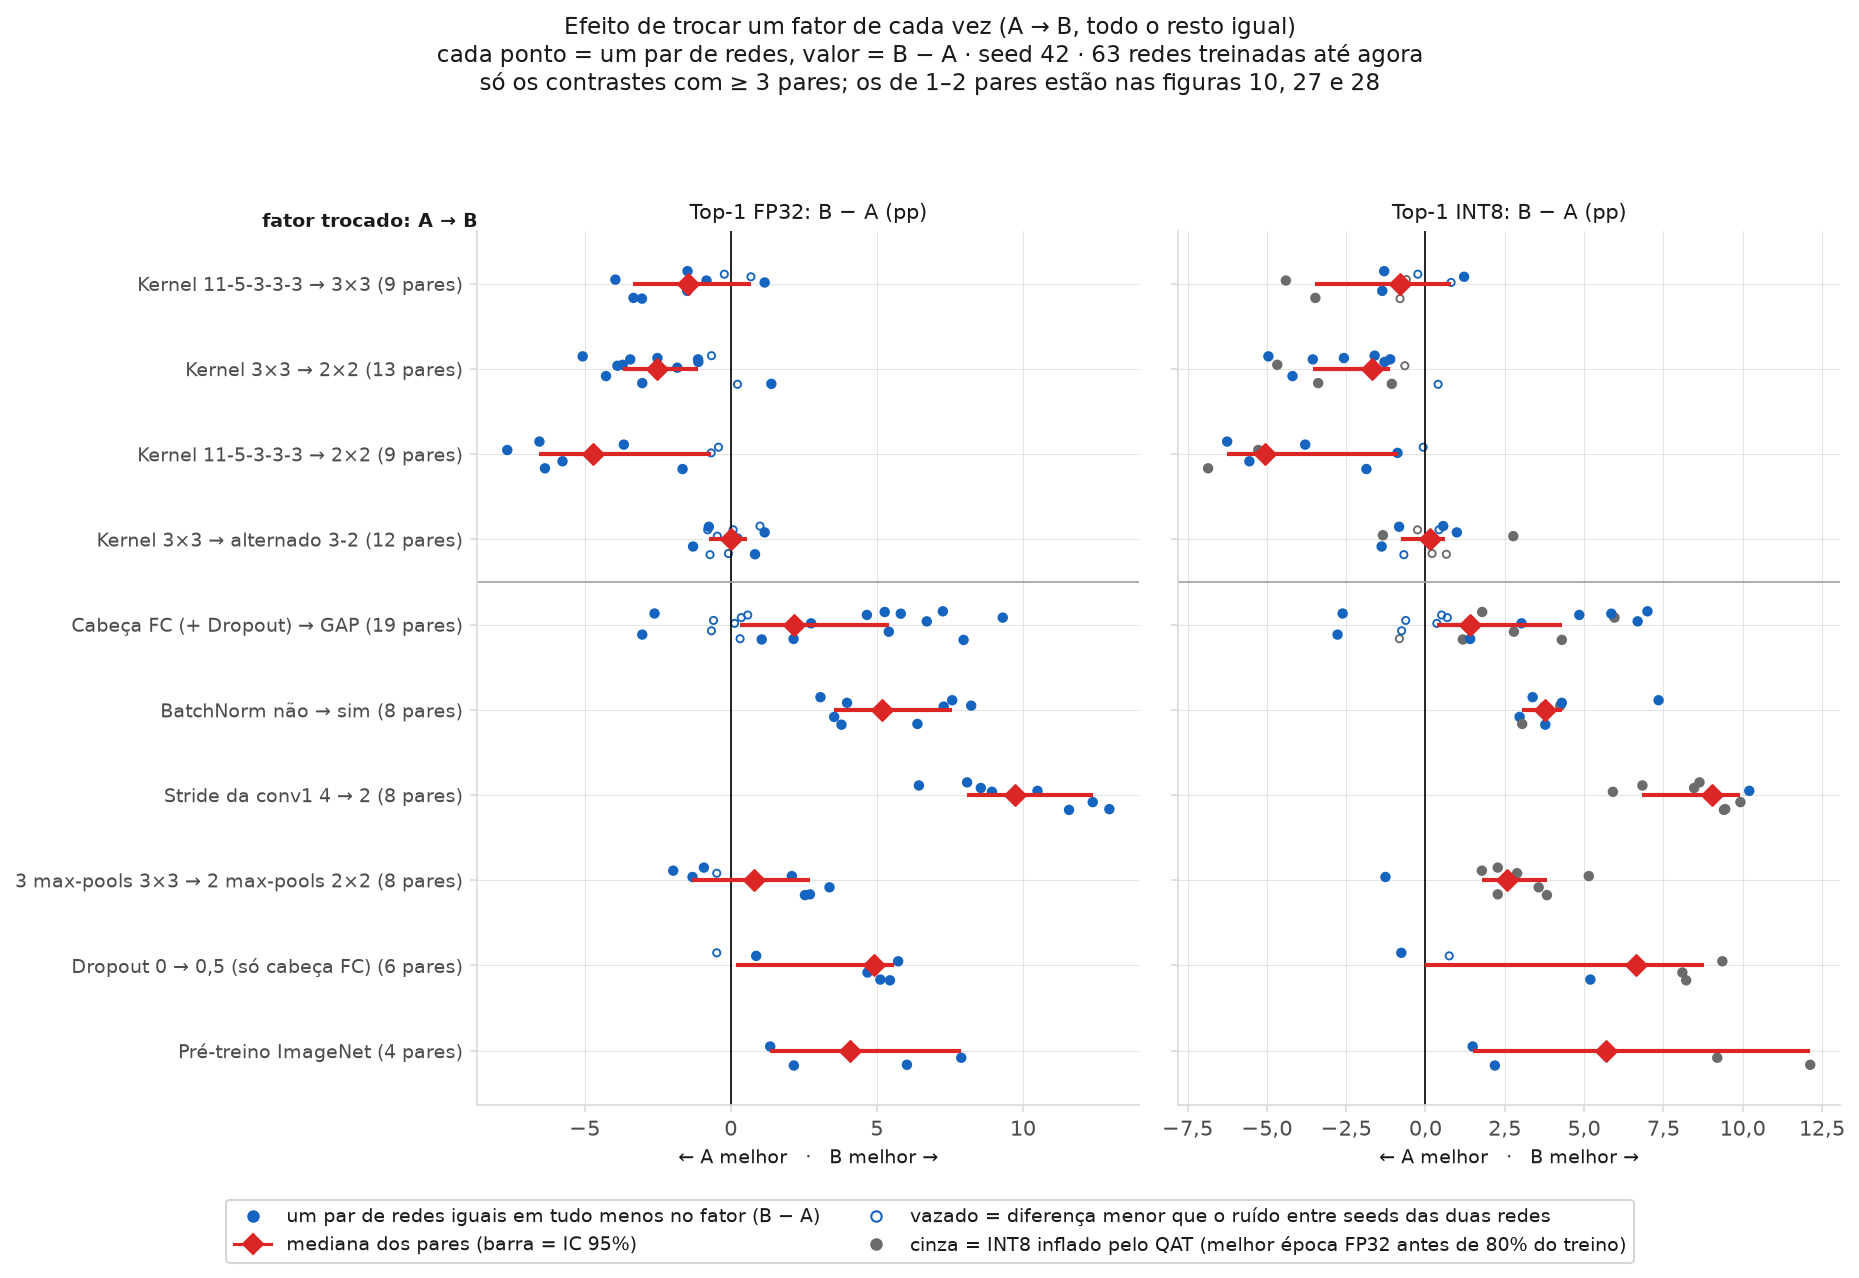
\includegraphics[width=\textwidth,trim=0 0 0 49,clip]{phase_11_kernel_size_comparison/11_factorial_matched_pairs.png}
\caption{Efeito de trocar um fator de cada vez (seed 42). Cada ponto é um par de redes iguais no resto, com o valor B $-$ A. O losango é a mediana dos pares, e a barra, seu IC 95\%. Com dois pares não há barra: eles são a rede com GAP + BN e a com FC + Dropout + BN. No INT8, a mediana e o IC
deixam de fora os pares com anel (INT8 inflado pelo QAT). Pontos vazados estão dentro da variação entre seeds. As dez primeiras linhas são de kernel. À direita, o número de pares e a variação mediana de MACs (custo efetivo) e de parâmetros.}
\label{fig:pares}
\end{figure*}

As medianas, porém, misturam situações diferentes. A Tabela~\ref{tab:grade} separa as duas colunas com BN da AlexNet, e a Figura~\ref{fig:grade} mostra as quatro.

\begin{table}[!t]
\caption{AlexNet de layout 64 px com BN: acurácia FP32 (\%) e MACs por kernel}
\label{tab:grade}
\centering
\footnotesize
\setlength{\tabcolsep}{3pt}
\begin{tabular}{@{}lcccc@{}}
\toprule
 & \multicolumn{2}{c}{\textbf{GAP (3 seeds)}} & \multicolumn{2}{c}{\textbf{FC + Dropout (seed 42)}} \\
\textbf{Kernels} & \textbf{FP32} & \textbf{MACs} & \textbf{FP32} & \textbf{MACs} \\
\midrule
5\by5 & 49,25 & 464M & 52,14 & 519M \\
11-5-3-3-3 & 53,07 & 240M & 52,23 & 295M \\
3\by3 & 53,81 & 167M & 50,75 & 223M \\
Alternado 3-2 & 54,58 & 120M & 50,00 & 175M \\
2\by2 & 52,58 & 75M & 45,68 & 130M \\
\bottomrule
\end{tabular}
\end{table}

Com GAP e BN, os kernels pequenos quase não custam: o 3\by3 fica 0,74 p.p. acima do 11-5-3-3-3, e o alternado 3-2, 0,77 p.p. acima do 3\by3. O 2\by2 fica 1,23 p.p. abaixo do 3\by3, mas só 0,49 p.p. abaixo dos kernels originais, com 69\% menos MACs. Todas essas
diferenças passam da faixa de $\pm$0,4 p.p. para médias de 3 seeds.

Com FC, Dropout e BN, a ordem se inverte e passa a seguir o tamanho do kernel: o 2\by2 perde 5,1 p.p. para o 3\by3 e 6,5 p.p. para o 11-5-3-3-3. Sem BN, o FC + Dropout também penaliza o 2\by2 (39,60\%, contra 44,10\% do 11-5-3-3-3, 3 seeds). Não investigamos por que o classificador
FC favorece kernels maiores nessa rede.

\begin{figure*}[!t]
\centering
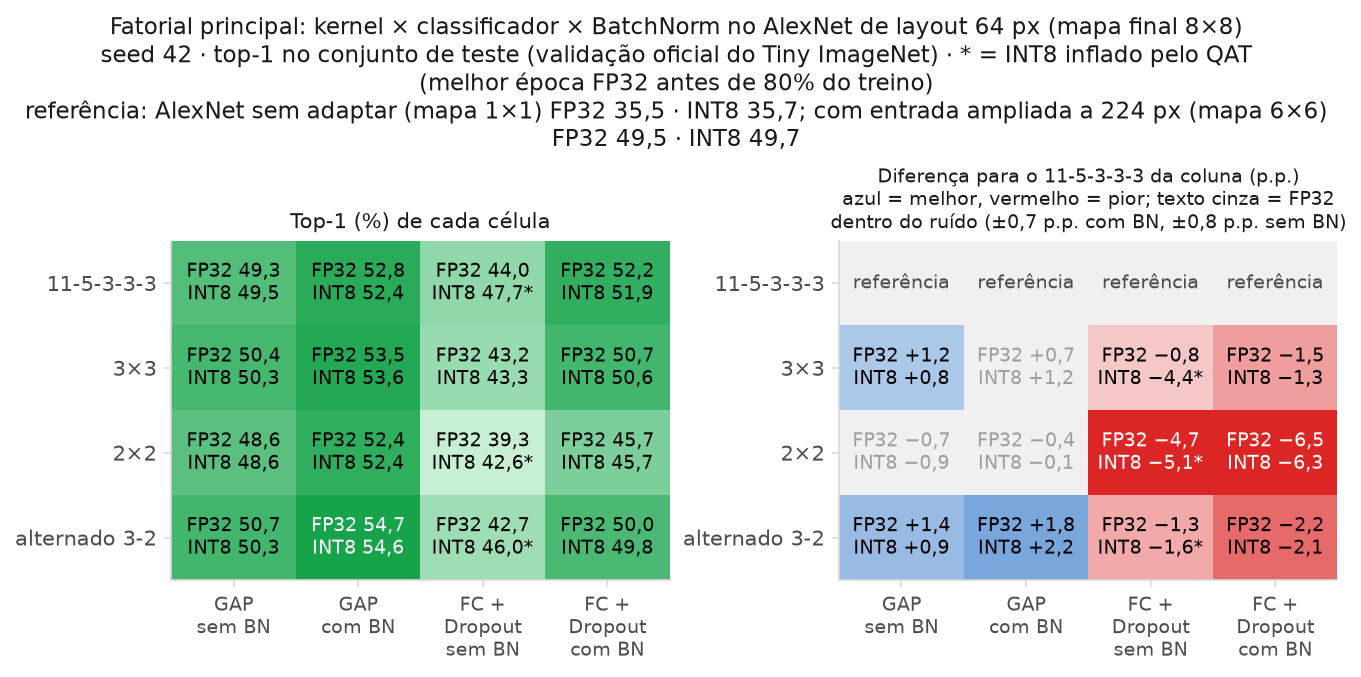
\includegraphics[width=\textwidth,trim=0 0 0 75.8,clip]{phase_11_kernel_size_comparison/14_main_factorial_grid.png}
\caption{Kernel, classificador e BN na AlexNet de layout 64 px (seed 42). À esquerda, a acurácia de cada combinação; à direita, a diferença para o
11-5-3-3-3 da mesma coluna. Com GAP (duas primeiras colunas), os kernels pequenos ficam perto do original ou acima dele. Cinza: dentro da variação entre seeds; asterisco: INT8 inflado pelo QAT. Para comparar: a AlexNet sem adaptação fica em 35,5\% em FP32, e com imagem ampliada para 224 px, em 49,5\%.}
\label{fig:grade}
\end{figure*}

A VGG16 se comporta ao contrário da AlexNet (Figura~\ref{fig:vgg}). Com GAP e BN, o 2\by2 custa 2,43 p.p. (56,84\% contra 59,27\%, 3 seeds); com FC e Dropout, empata (59,17\% contra 58,83\%, 3 seeds); e, com FC sem Dropout, fica 1,12 p.p. abaixo (uma seed). Na ResNet-18, que usa GAP e BN, o 2\by2 custa 1,01 p.p. em relação ao
3\by3 (41,86\% contra 42,87\%, 3 seeds). Portanto, a conclusão ``o FC agrava o custo do 2\by2'' vale para a AlexNet, não em geral.

\begin{figure*}[!t]
\centering
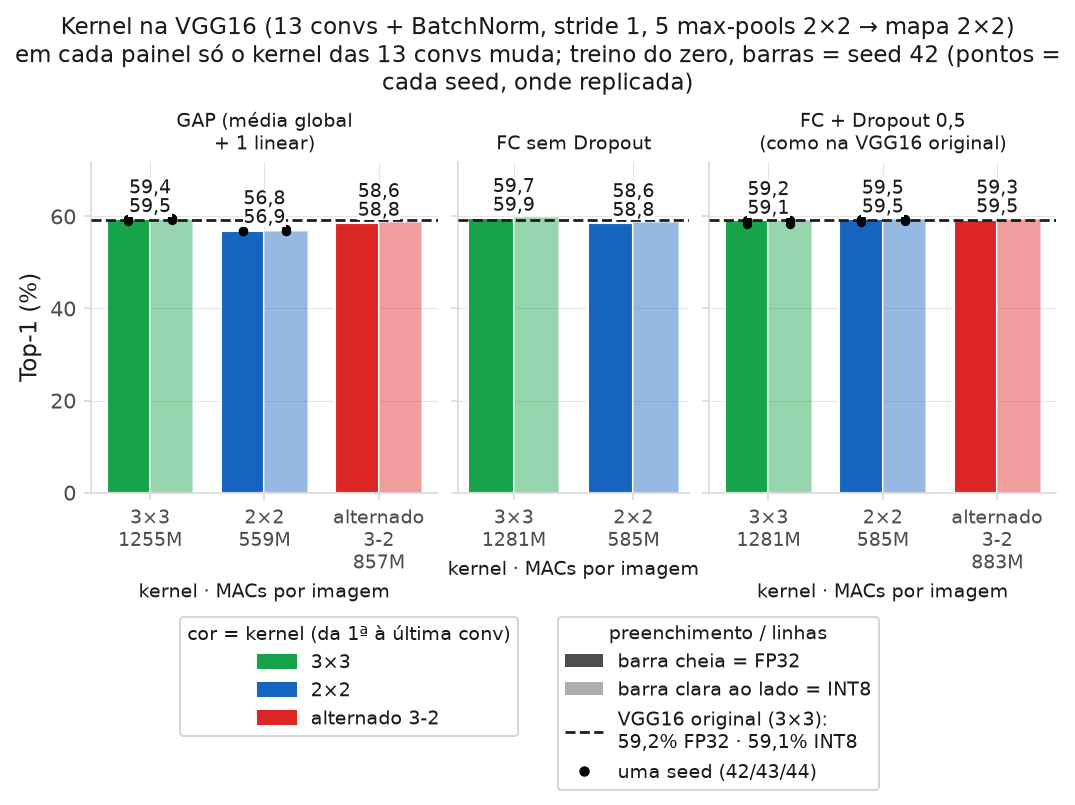
\includegraphics[width=0.86\textwidth,trim=0 0 0 49.4,clip]{phase_11_kernel_size_comparison/03_kernel_vgg16.png}
\caption{Kernel na VGG16 (13 convoluções, BN, do zero). Em cada painel, só o kernel das 13 convoluções muda. Barras: seed 42; pontos: cada seed, onde houver; linha tracejada: a VGG16 original (3\by3, FC + Dropout). O 2\by2 perde com GAP e, por menos, com FC sem Dropout (uma seed). Com FC + Dropout, empata.}
\label{fig:vgg}
\end{figure*}


\subsection{O 2\by2 perde pelo kernel ou pela capacidade?}
\label{sec:controles}

Na AlexNet com GAP e BN, o 2\by2 perde pela capacidade. Uma rede 2\by2 tem menos pesos e faz menos multiplicações que uma 3\by3 com os mesmos canais, e os controles de largura separam as duas coisas (Figura~\ref{fig:controles}a). Com os mesmos MACs e parâmetros, as redes empatam: 53,83\% contra 53,81\% com 167M de MACs, e
52,58\% contra 52,59\% com 75M (3 seeds cada). Esse controle não foi feito com FC, nem na VGG16 ou na ResNet-18; a perda maior do 2\by2 com FC na AlexNet, portanto, continua sem explicação.

No sentido oposto, kernels maiores não compram acurácia com GAP. Com 5\by5 em todas as convoluções, a rede custa 2,8 vezes o 3\by3 e chega a 49,25\%, ou 4,56 p.p. abaixo dele (3 seeds, Figura~\ref{fig:controles}b). Com GAP e BN, portanto, gastar mais só compensou como largura, não como kernel maior. Com FC + Dropout, o 5\by5 chega a 52,14\% (uma seed), perto dos 52,23\% do 11-5-3-3-3,
o que combina com o que a Tabela~\ref{tab:grade} já mostrou.

\begin{figure*}[!t]
\centering
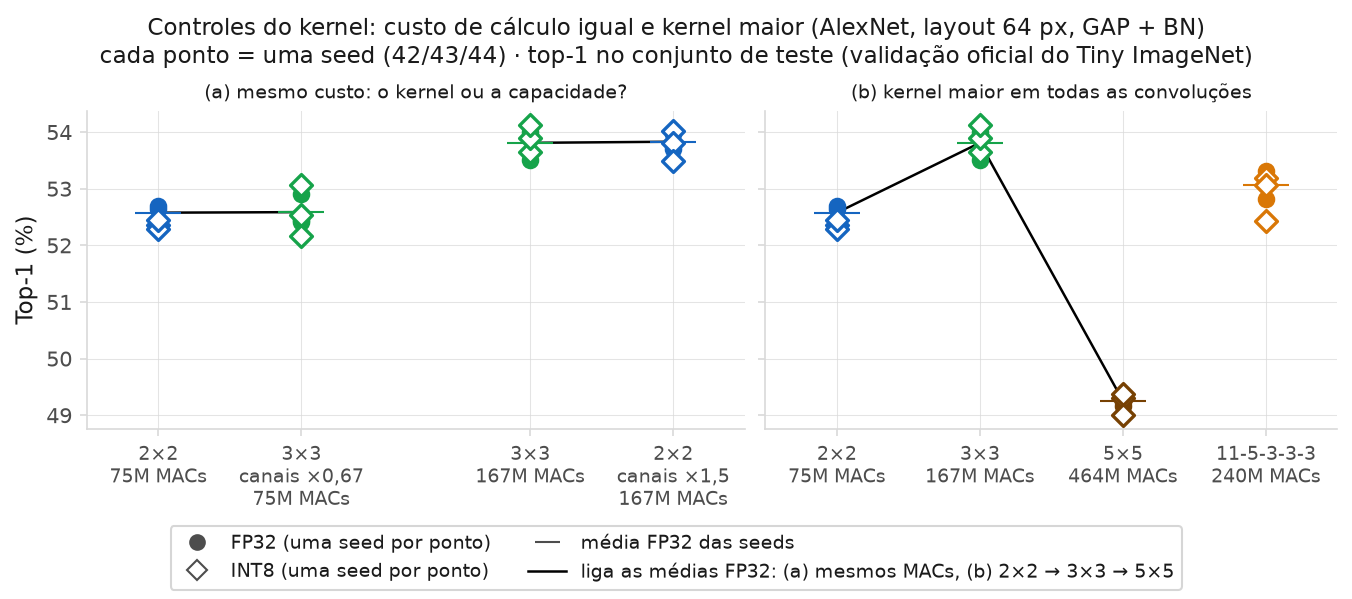
\includegraphics[width=\textwidth,trim=0 0 0 36,clip]{phase_11_kernel_size_comparison/26_kernel_controls.png}
\caption{(a) Com o mesmo custo em MACs, 2\by2 e 3\by3 empatam. (b) Um kernel maior não ajuda: o 5\by5 custa mais e fica bem abaixo do 3\by3.
Cada ponto é uma seed, com top-1 no teste. AlexNet de layout 64 px, GAP e BN.}
\label{fig:controles}
\end{figure*}

Resta saber em que parte da rede o 2\by2 custa. Na VGG16 com GAP e BN, trocamos o kernel de um bloco por vez (Tabela~\ref{tab:vggblocos}; Figura~\ref{fig:blocos}, no Apêndice). Colocar 2\by2 nos blocos 1, 2, 3 ou 5 fica dentro da faixa de $\pm$0,5 p.p. para médias de 3 seeds. O bloco 4 é o único que sai dela: custa 0,71 p.p., um efeito pequeno e provável, já que fica pouco acima da faixa. A perda maior
só aparece quando todos os blocos usam 2\by2, ou seja, nenhum bloco sozinho concentra o custo.

\begin{table}[!t]
\caption{VGG16 com GAP e BN: 2\by2 em um bloco por vez (FP32, 3 seeds)}
\label{tab:vggblocos}
\centering
\footnotesize
\begin{tabular}{@{}lcc@{}}
\toprule
\textbf{Onde está o 2\by2} & \textbf{FP32 (\%)} & \textbf{Diferença para 3\by3 (p.p.)} \\
\midrule
Nenhum bloco (3\by3) & 59,27 & --- \\
Bloco 1 & 59,54 & $+$0,27 \\
Bloco 2 & 59,34 & $+$0,07 \\
Bloco 3 & 59,05 & $-$0,22 \\
Bloco 4 & 58,56 & $-$0,71 \\
Bloco 5 & 59,18 & $-$0,09 \\
Todos os blocos & 56,84 & $-$2,43 \\
\bottomrule
\end{tabular}
\end{table}

\FloatBarrier

\subsection{Dá para recuperar a perda sem um corpo de kernel grande?}
\label{sec:recuperar}

Sim, de duas formas: mantendo um kernel grande só na conv1 ou usando duas convoluções pequenas por estágio. Testamos as duas na AlexNet de layout 64 px.

A primeira é a conv1 11\by11 com corpo pequeno (Figura~\ref{fig:conv1}). Com corpo 2\by2, essa rede chega a 55,93\% em FP32 e 56,11\% em INT8 (3 seeds), com 98M de MACs, e supera o 3\by3 (53,81\%, 167M) e os kernels originais (53,07\%, 240M). Como a conv1 tem stride 2, ela já estaria fora de um acelerador de Winograd com qualquer kernel. Ainda assim, há um preço: com a
conv1 maior, a parcela dos MACs que o acelerador pode executar cai de 98,4\% para 75,2\%.

\begin{figure*}[!t]
\centering
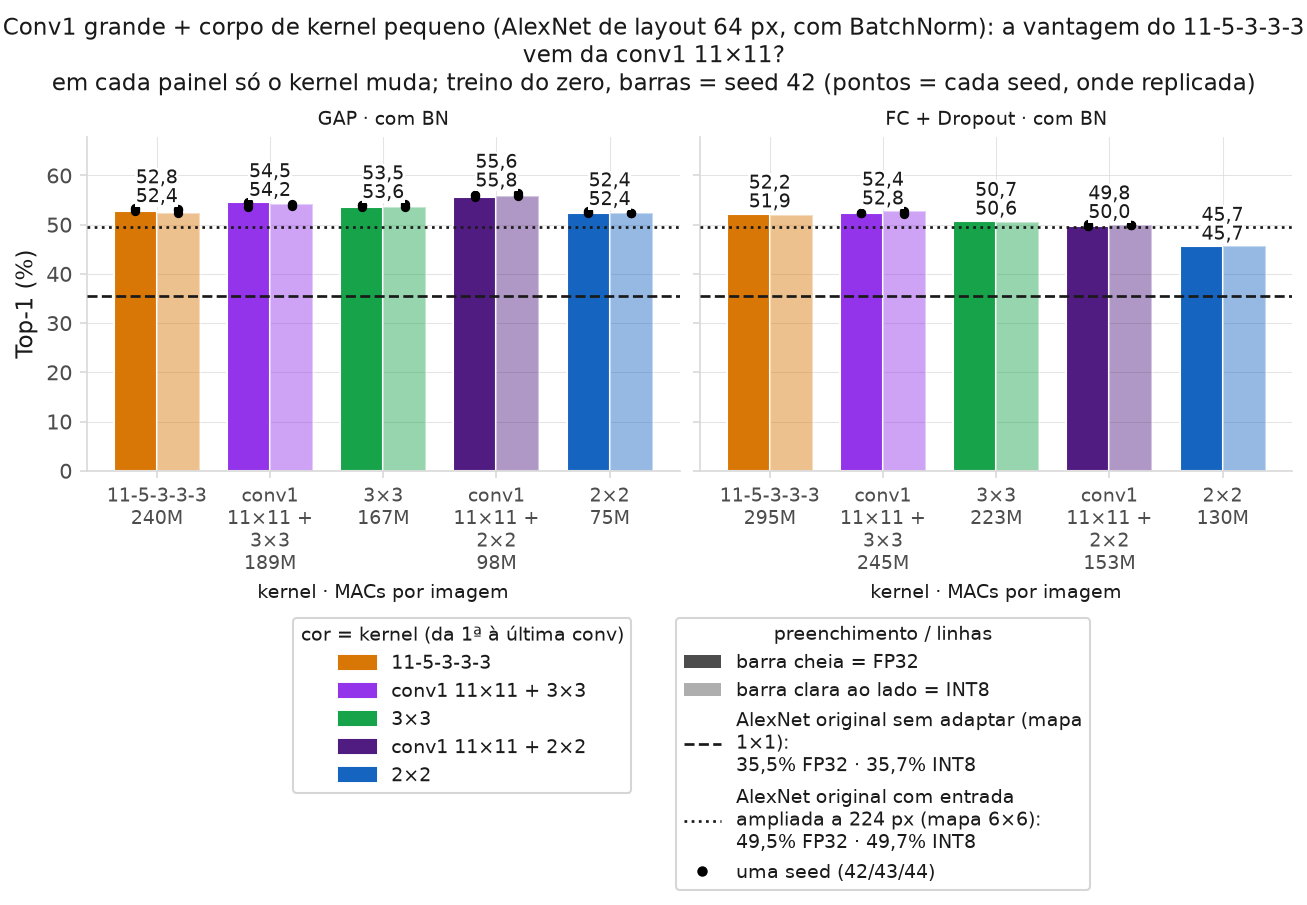
\includegraphics[width=\textwidth,trim=0 0 0 49.4,clip]{phase_11_kernel_size_comparison/27_large_stem.png}
\caption{Conv1 grande com corpo de kernel pequeno, com BN, do zero. Com GAP (à esquerda), a conv1 11\by11 com corpo 2\by2 é a melhor das cinco e a segunda mais barata. Barras: seed 42 (cheia: FP32; clara: INT8), por isso diferem das médias do texto; pontos: cada seed. Linhas: a AlexNet sem adaptação (tracejada) e com a imagem ampliada para 224 px (pontilhada).}
\label{fig:conv1}
\end{figure*}

A segunda forma são duas convoluções pequenas por estágio. Aqui o ganho depende do classificador, e por isso as medianas da Figura~\ref{fig:pares} ($+$5,3 e $+$8,0 p.p.) precisam ser lidas com cuidado, já que cada uma resume dois pares. Com GAP e BN, a configuração que recomendamos, o ganho é de $+$2,37 p.p. no 3\by3 e $+$4,86 p.p. no 2\by2 (seed 42, como na Figura~\ref{fig:pares}); com FC + Dropout + BN, é de
$+$8,15 e $+$11,21 p.p. Em troca, os MACs sobem 169\% com GAP e BN, e 127\% (3\by3) e 97\% (2\by2) com FC. Com GAP e BN, a rede 2\by2 com dois por estágio (57,25\%, 201M) fica até acima da 3\by3 equivalente (55,87\%, 451M), com uma seed cada.

O campo receptivo efetivo dá uma pista de por que dois por estágio ajudam (Figura~\ref{fig:erf}): a área com metade da influência vai de 17,8\% para 29,8\% da imagem no 2\by2, e de 23,5\% para 33,1\% no 3\by3. Já a conv1 11\by11 quase não amplia essa área (18,5\% contra 17,8\%), embora melhore a acurácia. Seu ganho, portanto, não parece
vir de enxergar mais da imagem, e não testamos a causa.

\begin{figure*}[!t]
\centering
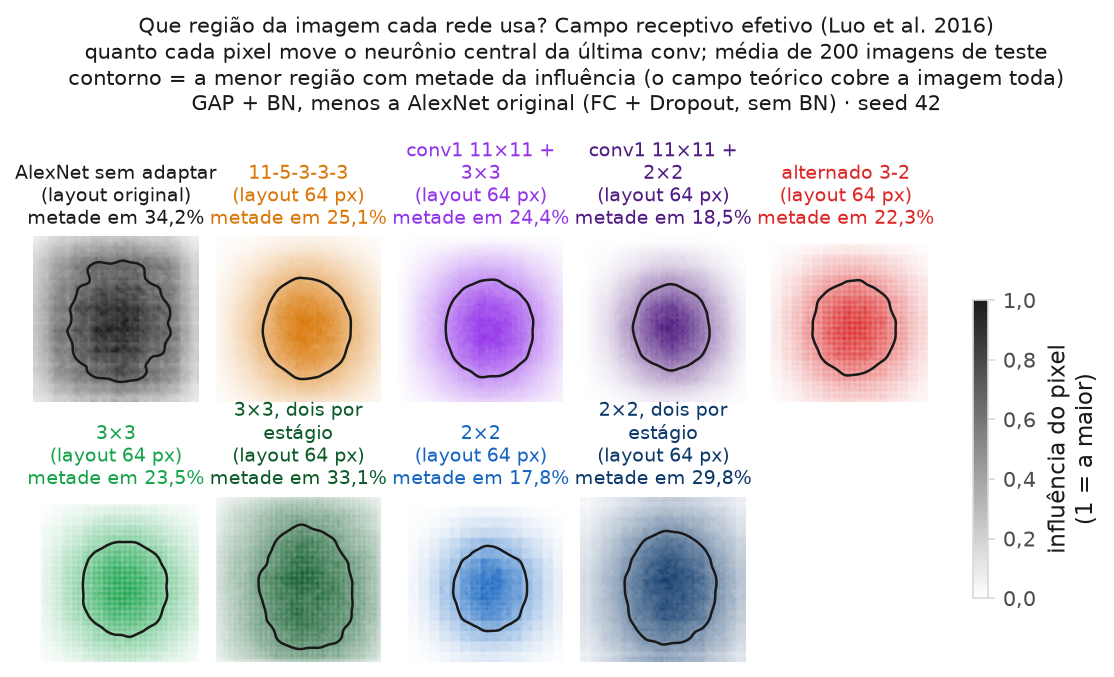
\includegraphics[width=0.8\textwidth,trim=0 0 0 61.4,clip]{phase_11_kernel_size_comparison/22_effective_receptive_field.png}
\caption{Que região da imagem cada rede usa: quanto cada pixel move a unidade central da última convolução (média de 200 imagens de teste, seed 42). O contorno marca a menor região com metade da influência. Todas têm GAP e BN e o layout de 64 px, menos a AlexNet original (FC + Dropout, sem BN, layout original). Compare, na segunda linha, cada kernel com sua versão de dois por estágio.}
\label{fig:erf}
\end{figure*}


\subsection{A quantização INT8 atrapalha?}
\label{sec:int8}

A quantização quase não altera a acurácia, e o tamanho do kernel não muda esse quadro (Figura~\ref{fig:int8}). Comparando o FP32 e o INT8 de cada rede no mesmo conjunto de teste, a diferença nos 126 treinos do estudo principal sem a marca de melhor época cedo vai de $-$0,38 a $+$0,58 p.p., com mediana de $+$0,04 p.p. No estudo de combinações, em que nenhum treino recebeu a marca, ela vai de
$-$0,44 a $+$0,77 p.p.

Os ganhos grandes em INT8 aparecem apenas nos 26 treinos marcados, em que a diferença vai de $+$0,56 a $+$6,69 p.p., e não são efeito da quantização: ali o QAT continua treinando, agora com uma taxa de aprendizado baixa, uma rede que ainda não tinha terminado de convergir.

\begin{figure*}[!t]
\centering
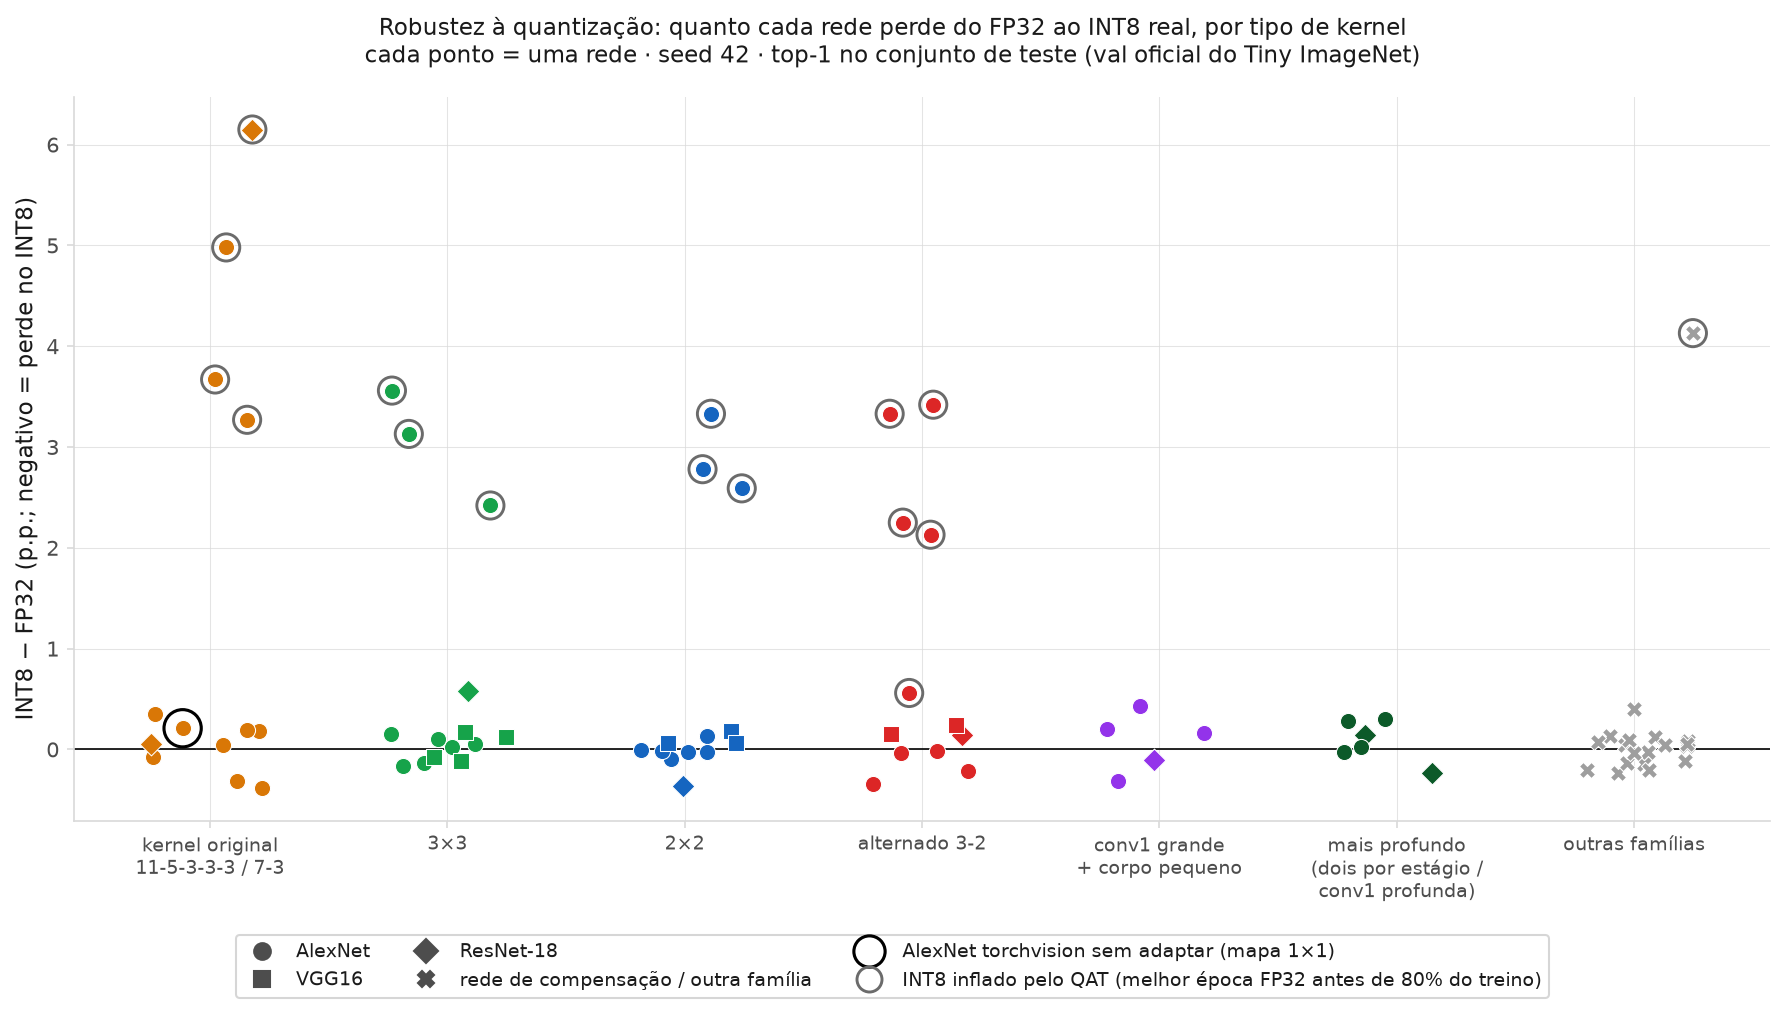
\includegraphics[width=\textwidth,trim=0 0 0 36,clip]{phase_11_kernel_size_comparison/16_quantization_robustness.png}
\caption{Quanto cada rede muda do FP32 para o INT8, por tipo de kernel (seed 42, top-1 no teste). Valores negativos indicam perda em INT8. Sem a marca do anel, todas as redes ficam perto de zero, seja qual for o kernel. Os pontos altos, com anel, são treino extra do QAT. O quadrado marca a AlexNet sem adaptação. Grupos: original = 11-5-3-3-3 ou 7-3 (ResNet-18); conv1 grande = conv1 11\by11 ou 7\by7 com corpo pequeno; 2 por estágio inclui a conv1 profunda da ResNet-18; outras = redes de compensação e MobileNetV2.}
\label{fig:int8}
\end{figure*}

Acurácia igual, porém, não quer dizer respostas iguais \cite{hooker2019what}. A maioria das redes troca de 2\% a 7\% das imagens de teste entre certo e errado, em quantidades parecidas nas duas direções, enquanto as redes marcadas chegam, em geral, a 9--14\% e quase sempre ganham no saldo (Figura~\ref{fig:flips}, no Apêndice).

A exceção é a MobileNetV2 pré-treinada. Nos três treinos dela, a concordância entre QAT e INT8 ficou abaixo da guarda de 0,90 (0,859, 0,888 e 0,899); como esses treinos terminaram com erro depois de salvar os resultados, seus números não passaram na nossa verificação. Com ajuste fino, ela perde 1,49 p.p. do FP32 para o INT8 (taxa
10$^{-4}$) e 1,16 p.p. (taxa 10$^{-3}$, treino marcado), ao passo que, fora ela, nenhum treino sem marca dos dois primeiros estudos perde mais de 0,38 p.p. A MobileNetV2 treinada do zero passa na guarda (0,94) e quase não muda (47,83\% para 47,88\%). A rede pré-treinada é a única com pesos da ImageNet e convoluções \textit{depthwise}, mas não investigamos a causa.


\subsection{Quanto da rede cabe em um acelerador Winograd?}
\label{sec:hardware}

A resposta depende da família, e uma rede barata não é necessariamente adequada ao acelerador. As Figuras~\ref{fig:pareto} e~\ref{fig:winograd} comparam acurácia e custo, e nelas a linha tracejada liga as redes que nenhuma outra supera nos dois critérios ao mesmo tempo. Na parte barata, ela passa por redes de compensação, como a Bottleneck; na intermediária, pela conv1 11\by11 com corpo 2\by2 e pela 2\by2 com dois por
estágio; e, na parte cara, pela VGG16. Isso vale para o estudo principal: as redes de stride 1 do estudo de combinações (Seção~\ref{sec:combinacoes}) passam a VGG16 com menos MACs (Tabela~\ref{tab:winograd}).

\begin{figure*}[!t]
\centering
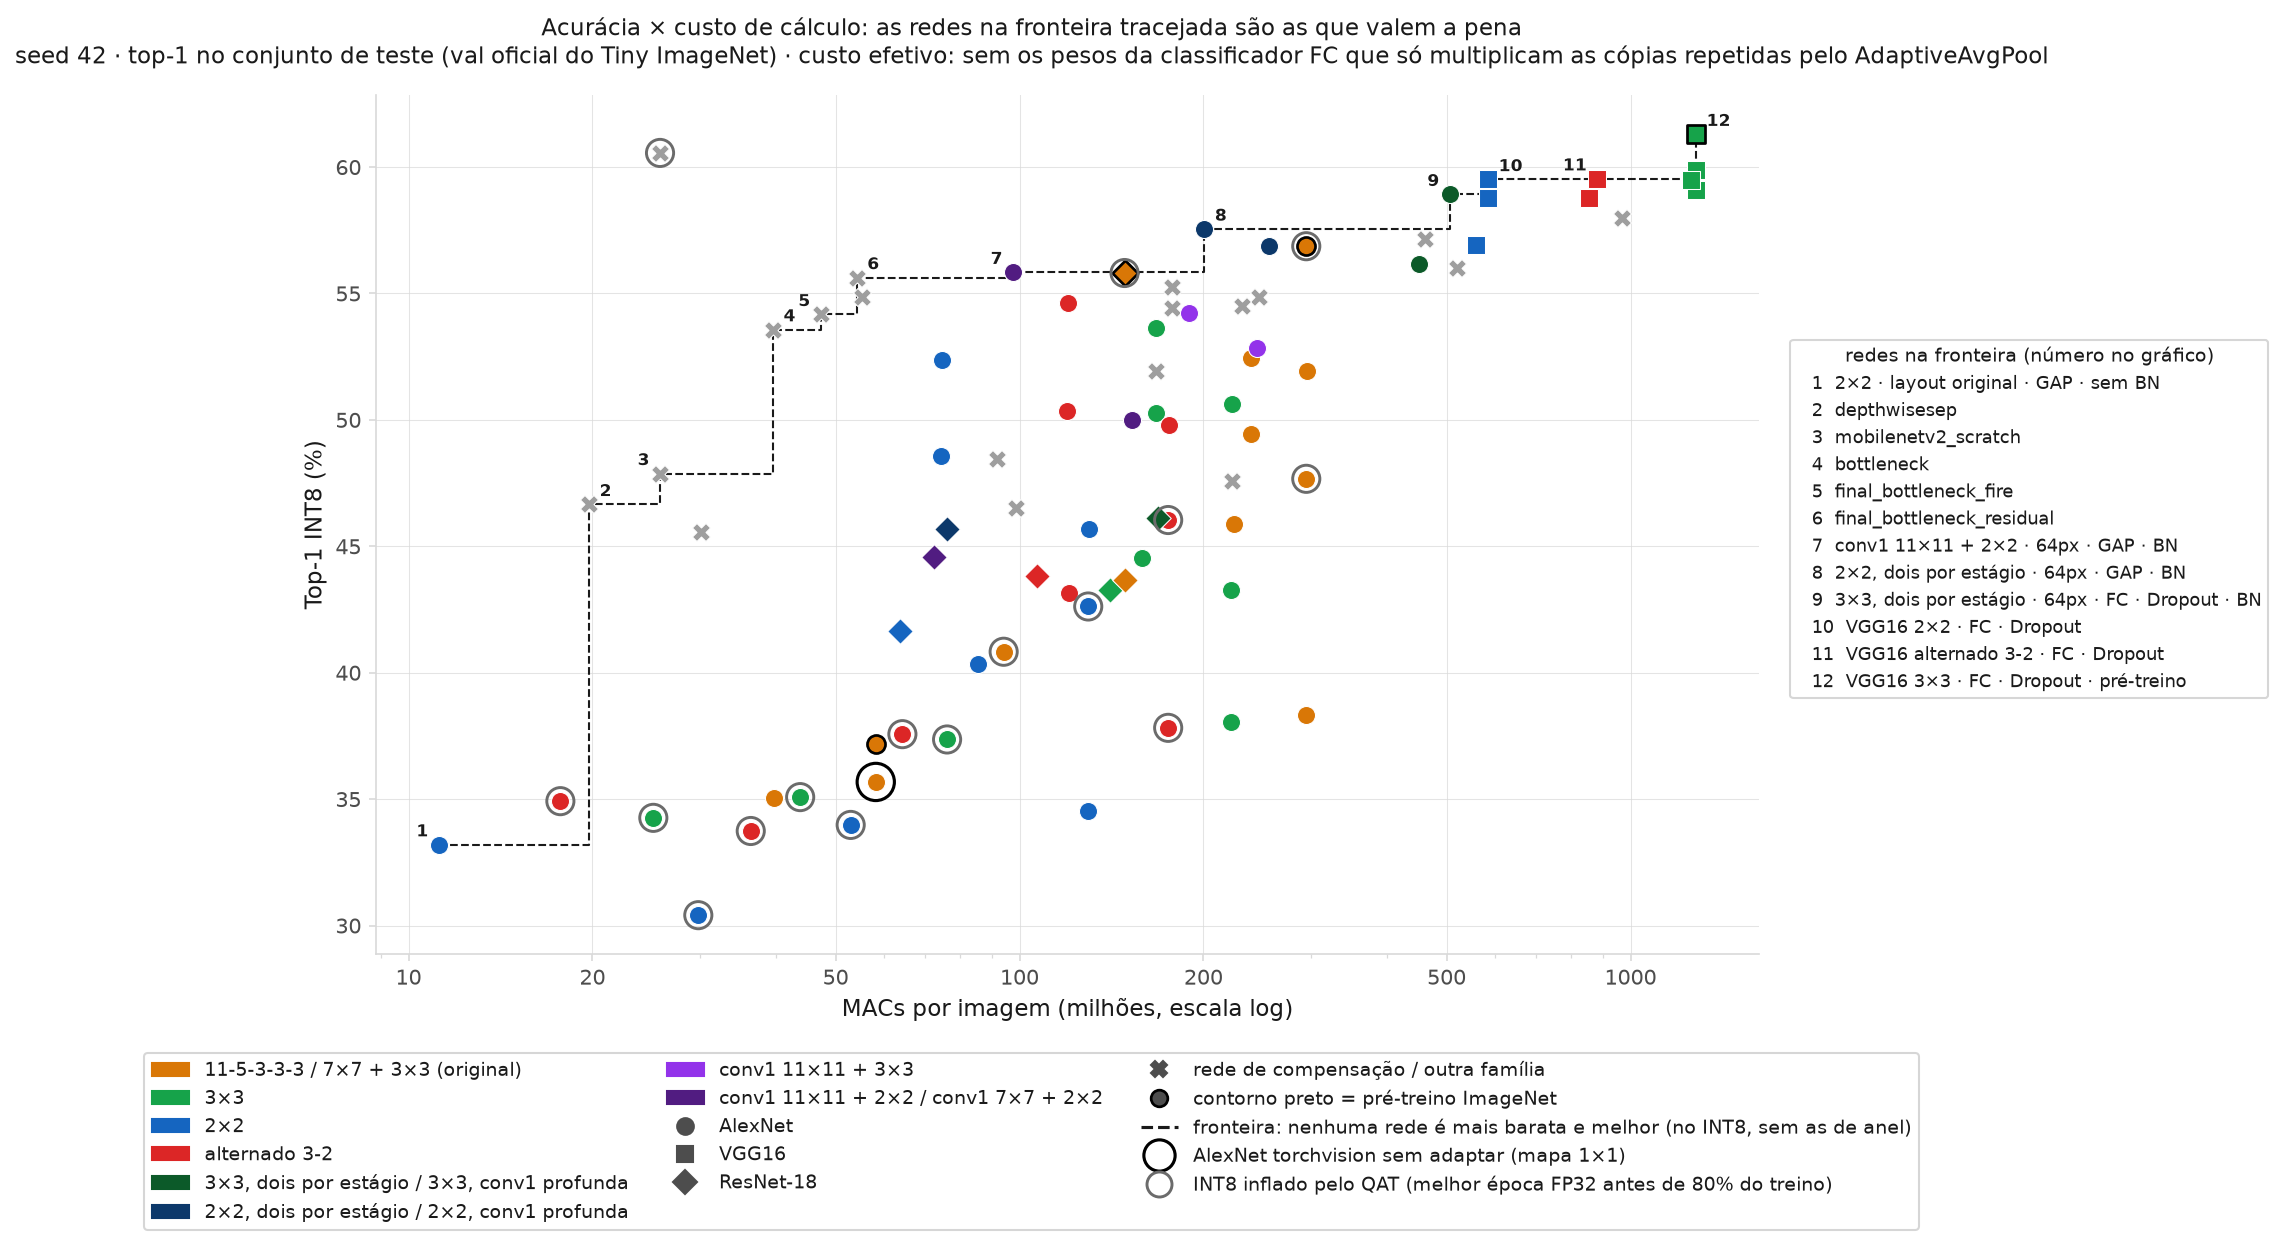
\includegraphics[width=\textwidth,trim=0 0 0 49.4,clip]{phase_11_kernel_size_comparison/13_pareto_accuracy_cost.png}
\caption{Acurácia INT8 e custo efetivo em MACs (estudo principal, seed 42). A linha tracejada liga as redes que nenhuma outra supera nos dois critérios ao mesmo tempo; as redes com anel ficam fora dela, porque seu INT8 está inflado pelo QAT. O quadrado marca a AlexNet sem adaptação.}
\label{fig:pareto}
\end{figure*}

\begin{figure*}[!t]
\centering
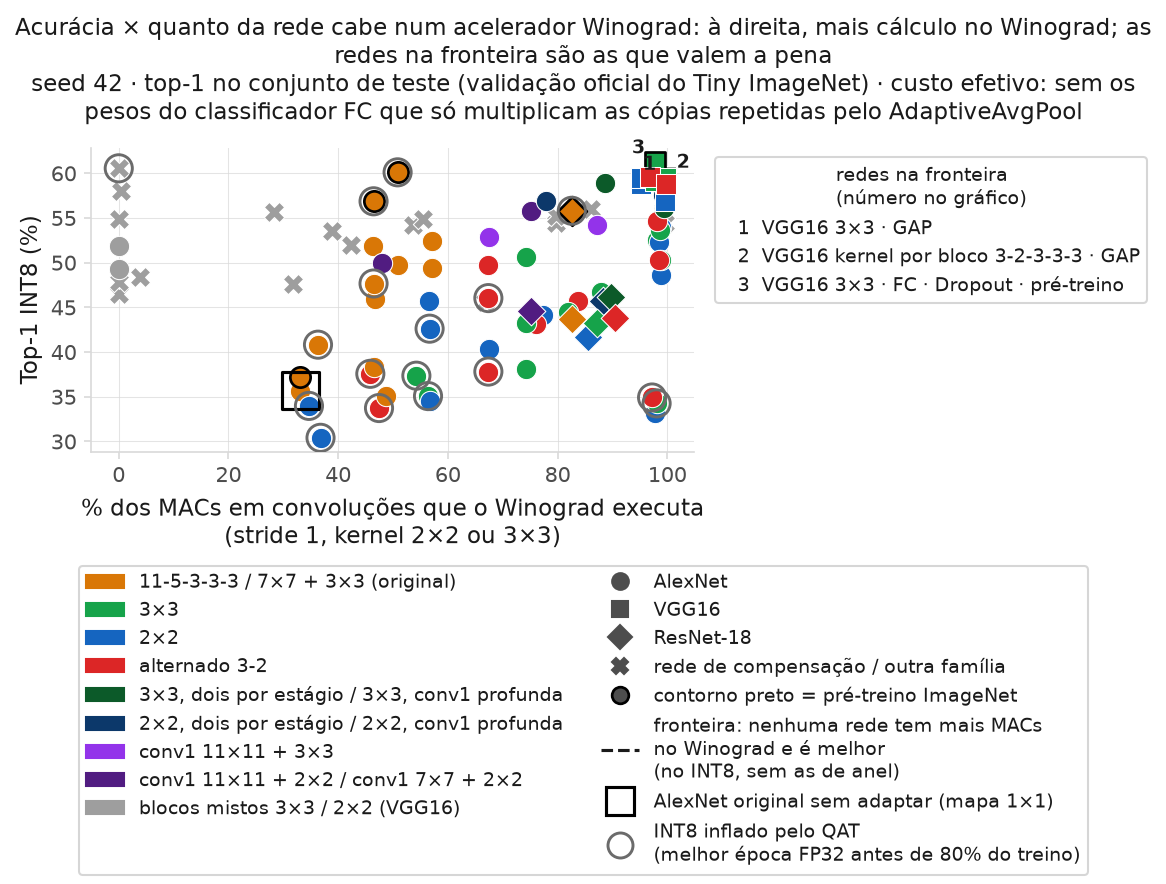
\includegraphics[width=\textwidth,trim=0 0 0 62.9,clip]{phase_11_kernel_size_comparison/30_winograd_eligible.png}
\caption{Acurácia INT8 e parcela dos MACs em convoluções que um acelerador Winograd pode executar (stride 1, kernel 2\by2 ou 3\by3, sem grupos; seed 42, custo efetivo). A linha tracejada liga as redes que nenhuma outra supera nos dois critérios (sem as de anel). Sem contar as redes com anel, as mais precisas, no canto superior direito, cabem quase inteiras. A conta usa só a geometria das camadas. Além das redes da Figura~\ref{fig:pareto}, entram as de imagem ampliada para 224 px e as VGG16 com um kernel por bloco (cinza).}
\label{fig:winograd}
\end{figure*}

A Tabela~\ref{tab:winograd} mostra a parcela dos MACs que o acelerador pode executar. As AlexNets de kernel pequeno e a VGG16 ficam perto de 100\%, enquanto a TinyMobileNetV2 e a MobileNetV2 ficam em torno de zero, e a FinalBottleneckResidual, em 28\%. Essas últimas economizam parâmetros ou MACs, mas gastam a maior parte do cálculo em convoluções 1\by1, \textit{depthwise} ou de stride maior que 1,
que o acelerador não aproveita \cite{souza2026relatorio}. A busca por uma rede eficiente e a busca por uma rede para Winograd levam, portanto, a escolhas diferentes; os blocos Fire sobre o melhor corpo ficam no meio do caminho (Seção~\ref{sec:unidades}).

\begin{table}[!t]
\caption{Acurácia, custo e parcela dos MACs que o acelerador pode executar (seed 42)}
\label{tab:winograd}
\centering
\footnotesize
\setlength{\tabcolsep}{3pt}
\begin{tabular}{@{}lccccc@{}}
\toprule
\textbf{Rede} & \textbf{FP32} & \textbf{INT8} & \textbf{Parâm.} & \textbf{MACs} & \textbf{Winograd} \\
 & \textbf{(\%)} & \textbf{(\%)} & \textbf{(M)} & \textbf{(M)} & \textbf{(\%)} \\
\midrule
2\by2, 2/est., atalho, stride 1 & 60,75 & 60,46 & 2,52 & 862 & 92,9 \\
2\by2, 2/est., stride 1 & 60,35 & 60,79 & 2,33 & 803 & 99,6 \\
VGG16 3\by3 & 59,35 & 59,47 & 14,82 & 1255 & 99,8 \\
TinyMobileNetV2 & 57,96 & 58,00 & 1,51 & 969 & 0,4 \\
2\by2, 2/est. & 57,25 & 57,55 & 2,33 & 201 & 99,2 \\
SmallKernel + BN & 57,20 & 57,17 & 1,60 & 461 & 99,7 \\
FinalBottleneckResidual & 55,83 & 55,63 & 0,57 & 54 & 28,3 \\
Conv1 11\by11 + corpo 2\by2 & 55,64 & 55,84 & 1,08 & 98 & 75,2 \\
FireBypass & 55,19 & 55,27 & 0,52 & 178 & 79,7 \\
Fire & 54,57 & 54,44 & 0,52 & 178 & 79,7 \\
Bottleneck & 53,71 & 53,57 & 0,39 & 40 & 38,8 \\
3\by3 & 53,50 & 53,65 & 2,30 & 167 & 98,7 \\
11-5-3-3-3 & 52,81 & 52,43 & 2,52 & 240 & 57,1 \\
2\by2 & 52,39 & 52,36 & 1,05 & 75 & 98,4 \\
MobileNetV2 (do zero) & 47,83 & 47,88 & 2,48 & 26 & 0,0 \\
DepthwiseSep & 46,53 & 46,66 & 0,31 & 20 & 0,0 \\
\bottomrule
\multicolumn{6}{@{}p{\linewidth}@{}}{\footnotesize 2/est. = dois por estágio. A coluna Winograd conta 2\by2 e 3\by3. Em um acelerador só com F($m$,3), as redes 2\by2 ficam perto de zero.}
\end{tabular}
\end{table}

É preciso lembrar que os MACs contam o método direto. Com Winograd, a vantagem do 2\by2 diminui, porque esse kernel economiza menos (Seção~\ref{sec:fundamentos}). Fizemos uma estimativa com a fórmula $(m+r-1)^2$, aplicada só às convoluções elegíveis: com F(2,3), a rede 3\by3 com dois por estágio cai de 451M para cerca de 202M multiplicações e, com F(2,2), a rede 2\by2 equivalente cai de 201M para cerca de
114M. A vantagem do 2\by2 passa, assim, de 2,2 vezes para cerca de 1,8 vez. Note que, com F(2,3), a rede 3\by3 faz praticamente as mesmas multiplicações (202M) que a 2\by2 pelo método direto (201M). Essa conta é aritmética, não uma medição: ela ignora o custo das transformações e a precisão numérica, e supõe um acelerador com F(2,2).


\subsection{Os resultados valem em outras condições?}
\label{sec:robustez}

Em boa parte, sim, mas só testamos redes com GAP e BN: os testes de taxa de aprendizado e de CIFAR-100 usam essa configuração, e o custo maior do 2\by2 com FC na AlexNet não foi repetido fora do cenário original. A Figura~\ref{fig:cenarios} resume os cenários.

O custo do kernel se repete. Trocar 3\by3 por 2\by2 custa de 0,7 a 2,4 p.p. em FP32 em todos os cenários e quase nada quando os MACs são iguais. Trocar os kernels originais por 3\by3 empata ou melhora um pouco nos cenários com AlexNet; na ResNet-18, a mesma troca fica em $-$0,95 p.p., dentro da faixa de uma seed.

\begin{figure*}[!t]
\centering
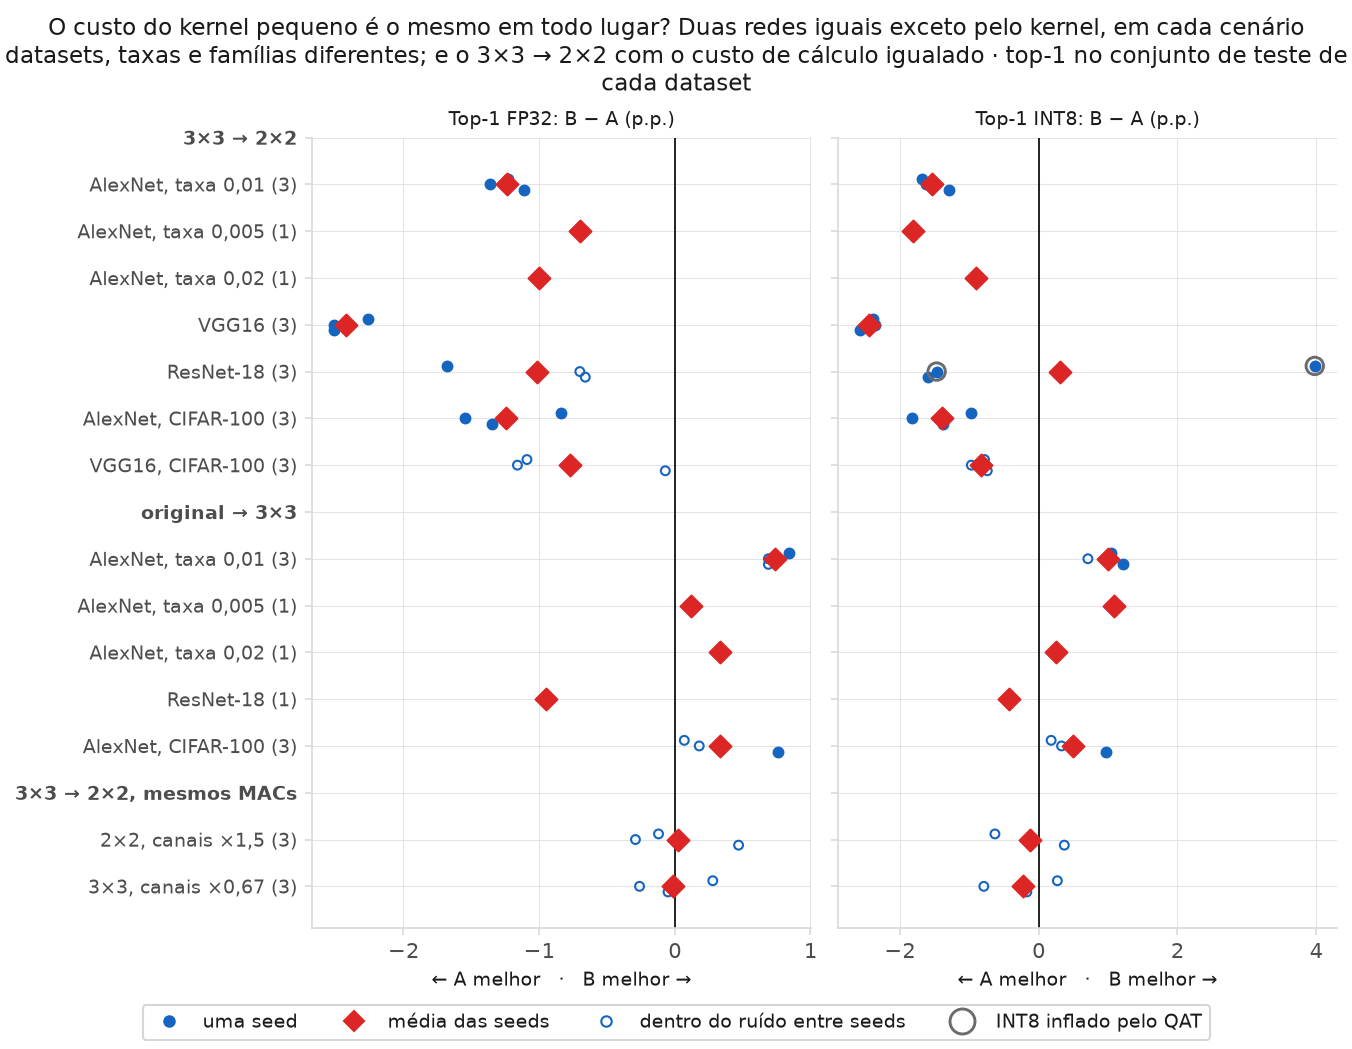
\includegraphics[width=\textwidth,trim=0 0 0 48.5,clip]{phase_12_robustness/04_kernel_effect_everywhere.png}
\caption{O efeito do kernel em cada cenário: duas redes iguais exceto pelo kernel (top-1 no teste de cada conjunto de dados: Tiny ImageNet, salvo onde diz CIFAR-100; entre parênteses, o número de seeds). O custo do 2\by2 aparece em todas as linhas do primeiro grupo e some no último, em que os MACs são iguais (o 2\by2 com 1,5 vez os canais, ou o 3\by3 com 0,67 vez). O grupo do meio compara os kernels originais (11-5-3-3-3 na AlexNet, 7\by7 na ResNet-18) com 3\by3. Um ponto muito à direita no INT8 da ResNet-18, com anel, é um caso de INT8 inflado pelo QAT.}
\label{fig:cenarios}
\end{figure*}

Com outras taxas de aprendizado (Tabela~\ref{tab:robustez}), a diferença entre 3\by3 e 11-5-3-3-3 fica dentro da faixa de uma seed nas taxas 0,005 e 0,02, então não afirmamos ordem entre eles. O 2\by2 fica abaixo do 3\by3 nas três taxas, de 0,7 a 1,1 p.p.; contra o 11-5-3-3-3, a diferença fica dentro da faixa nas taxas 0,005 e 0,02. Além disso, a taxa 0,02 fica acima da média das 3 seeds da taxa 0,01 nas três redes ($+$0,4 a $+$0,8 p.p., duas delas dentro da faixa), um sinal fraco de que a receita pode não ser a melhor para cada rede.

\begin{table}[!t]
\caption{Robustez: acurácia FP32 (\%) por kernel}
\label{tab:robustez}
\centering
\footnotesize
\setlength{\tabcolsep}{3pt}
\begin{tabular}{@{}lcccc@{}}
\toprule
\textbf{Cenário} & \textbf{11-5-3-3-3} & \textbf{3\by3} & \textbf{Alt. 3-2} & \textbf{2\by2} \\
\midrule
\multicolumn{5}{@{}l}{\textit{AlexNet, Tiny ImageNet, seed 42}} \\
Taxa 0,005 & 52,15 & 52,27 & --- & 51,57 \\
Taxa 0,01 (receita) & 52,81 & 53,50 & --- & 52,39 \\
Taxa 0,02 & 53,89 & 54,22 & --- & 53,22 \\
\midrule
\multicolumn{5}{@{}l}{\textit{CIFAR-100, 3 seeds}} \\
AlexNet & 63,00 & 63,34 & 63,42 & 62,09 \\
VGG16 & --- & 71,08 & 70,99 & 70,31 \\
\bottomrule
\end{tabular}
\end{table}

No CIFAR-100 (Tabela~\ref{tab:robustez}; Figura~\ref{fig:transferencia}, no Apêndice), a ordem dos kernels é a mesma do Tiny ImageNet nas duas famílias, com $\tau$ de Kendall igual a $+$1,00 \cite{kendall1938new}. Como são só quatro e três redes, e algumas ficam muito próximas, isso é um sinal de consistência, não uma prova.

Quanto ao pré-treino, a taxa de 0,01 da receita única apaga boa parte dele. Com ajuste fino de verdade \cite{li2020rethinking}, a taxa de 10$^{-3}$ supera a de 10$^{-4}$ em todas as redes testadas, e a VGG16 chega a 67,27\%; o ganho sobre a mesma rede treinada do zero vai de $+$5,5 a $+$14,9 p.p. em 64 px. Esse resultado, porém, não responde à pergunta sobre kernels, porque os
pesos pré-treinados só existem para os kernels originais de cada rede.


\subsection{Os ganhos se somam?}
\label{sec:combinacoes}

Os ganhos se somam apenas em parte. Testamos todas as combinações na AlexNet com GAP e BN: corpo 3\by3 ou 2\by2; conv1 com o kernel do corpo ou 11\by11; corpo de 5 convoluções, dois por estágio ou dois por estágio com atalho; stride da conv1 igual a 2 ou 1. São 24 redes, com a seed 42 (Figura~\ref{fig:hibridos}, Tabela~\ref{tab:combinacoes}).

\begin{figure*}[!t]
\centering
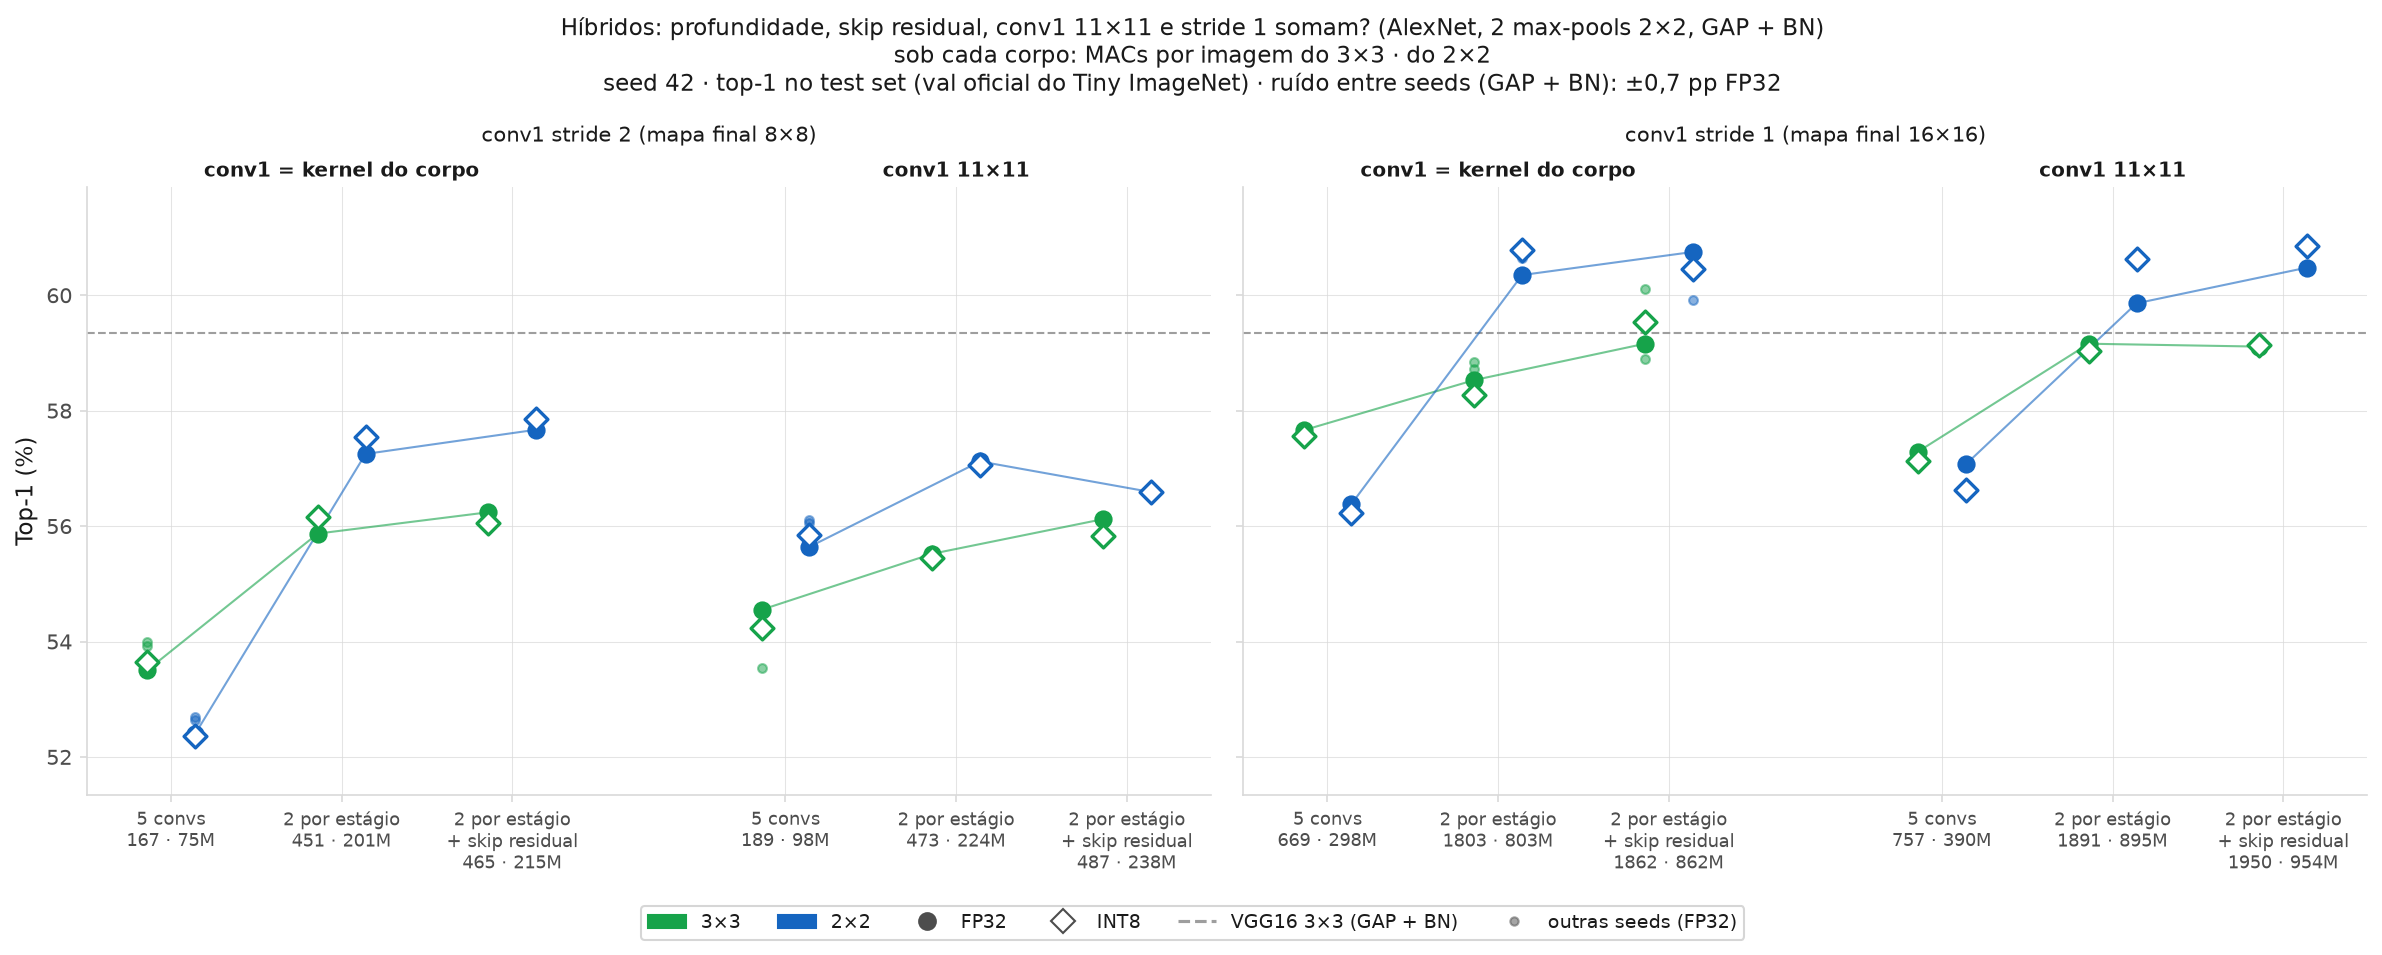
\includegraphics[width=\textwidth,trim=0 0 0 61.4,clip]{phase_13_hybrids/01_hybrids.png}
\caption{Todas as combinações (AlexNet com GAP e BN, seed 42; variação de um treino: $\pm$0,7 p.p. em FP32). Da esquerda para a direita, em cada grupo, o corpo fica mais profundo. O painel da direita (stride 1, mapa final 16\by16) fica acima do da esquerda (stride 2, mapa final 8\by8), e o azul (2\by2) passa o verde (3\by3) quando há dois kernels por estágio. A linha tracejada é a VGG16 3\by3. Os pontos pequenos são as seeds 43 e 44, onde houver. Sob cada corpo estão os MACs do 3\by3 e, abaixo, os do 2\by2.}
\label{fig:hibridos}
\end{figure*}

\begin{table}[!t]
\caption{Efeito de cada fator nas 24 combinações: mediana de B $-$ A (seed 42, p.p.)}
\label{tab:combinacoes}
\centering
\footnotesize
\setlength{\tabcolsep}{3pt}
\begin{tabular}{@{}lcccc@{}}
\toprule
\textbf{A $\rightarrow$ B} & \textbf{FP32} & \textbf{INT8} & \textbf{B acima} & \textbf{Faixa FP32} \\
\midrule
Stride da conv1: 2 $\rightarrow$ 1 & $+$3,03 & $+$3,40 & 12 de 12 & $+$1,43 a $+$4,16 \\
5 convs $\rightarrow$ 2 por estágio & $+$2,12 & $+$2,21 & 8 de 8 & $+$0,87 a $+$4,86 \\
Corpo 3\by3 $\rightarrow$ 2\by2 & $+$1,23 & $+$1,50 & 9 de 12 & $-$1,28 a $+$1,82 \\
2 por estágio $\rightarrow$ + atalho & $+$0,41 & $+$0,16 & 6 de 8 & $-$0,53 a $+$0,63 \\
Conv1 $\rightarrow$ 11\by11 & $-$0,12 & $-$0,19 & 4 de 12 & $-$1,08 a $+$3,25 \\
\bottomrule
\end{tabular}
\end{table}

Dois fatores nunca falham: o stride 1, que é o maior e custa quatro vezes mais MACs, e dois por estágio, que vêm em seguida. Já o atalho residual fica dentro da variação entre seeds, e seu sinal muda entre os pares, enquanto a conv1 11\by11 só ajuda no corpo de 5 convoluções (3 de 4 pares): com dois por estágio, sua mediana é de $-$0,20 p.p., ou seja, a segunda convolução por estágio já entrega o que ela entregava.

O resultado mais curioso é o do kernel do corpo. Com 5 convoluções, a troca de 3\by3 por 2\by2 varia de $-$1,28 a $+$1,09 p.p. Com dois por estágio, o 2\by2 vence nos 8 pares (de $+$0,47 a $+$1,82 p.p., mediana de $+$1,4), com cerca de metade dos MACs, e seis desses 8 pares passam da faixa de $\pm$0,7 p.p. É um indício forte, mas de uma seed, e por isso repetimos os dois pares de stride 1 com as seeds 43 e 44. Sem atalho, o 2\by2 vence nas três seeds (de $+$1,68 a $+$1,82 p.p. em FP32). Com atalho, vence em duas de três ($+$1,59, $+$1,48 e $-$0,18 p.p.): a 3\by3 com atalho da seed 44 (60,10\%) é a única dessas redes 3\by3 acima de 59,2\%, e sozinha fecha a diferença. A vantagem do 2\by2 com dois por estágio é, portanto, de cerca de 1 a 2 p.p., mas não é firme nos dois corpos.

Os dois maiores ganhos, por sua vez, não se somam por inteiro. Partindo do 3\by3 com stride 2 (53,50\%), os ganhos separados de usar dois por estágio ($+$2,37) e stride 1 ($+$4,16) levariam a 60,03\%, mas o valor medido é 58,53\%. No 2\by2, a soma levaria a 61,24\%, e o valor medido é 60,35\%: o corpo 2\by2 perde menos nessa combinação.

As melhores redes usam corpo 2\by2, dois por estágio e stride 1. Só com 2\by2 e com atalho, a rede chega a 60,75\% em FP32 e 60,46\% em INT8 (2,52M de parâmetros, 862M de MACs); sem atalho, a 60,35\% e 60,79\% (2,33M, 803M). Com a conv1 11\by11 e atalho, chega a 60,48\% e 60,85\%, o maior INT8 das 24, empatada com as outras duas. A VGG16 3\by3 com GAP e BN fica em 59,35\% e 59,47\%, com 14,82M de parâmetros e 1255M de MACs (de 59,09\% a 59,37\% em FP32, em 3 seeds). As duas AlexNets só com 2\by2 ficam, assim,
de 1,0 a 1,4 p.p. acima dela, com cerca de um sexto dos parâmetros e dois terços dos MACs.

Como essas duas redes saíram do topo das 24, a seed 42 pode estar favorecendo as duas, e por isso as repetimos com as seeds 43 e 44. Nas médias de 3 seeds, a rede sem atalho fica em 60,47\% (FP32) e 60,63\% (INT8), e a com atalho em 60,35\% e 60,34\%, contra 59,27\% e 59,45\% da VGG16. A pior seed de cada uma (60,35\% sem atalho e 59,92\% com atalho, em FP32) fica acima da melhor seed da VGG16 (59,37\%). O atalho continua sem efeito no corpo 2\by2 (média de $-$0,12 p.p. em FP32, com o sinal trocando entre as seeds). No corpo 3\by3, ele é positivo nas três seeds (média de $+$0,68 p.p.), mas vai de $+$0,05 a $+$1,37 p.p., e três seeds não bastam para medi-lo. Já as redes 3\by3 com dois por estágio não superam a VGG16 com clareza: 58,70\% sem atalho e 59,39\% com atalho em FP32.

\subsection{Blocos Bottleneck e Fire barateiam o melhor corpo?}
\label{sec:unidades}

A resposta é sim para o Fire com dois blocos por estágio; com um bloco por estágio, nenhum dos dois consegue. Para chegar a ela, partimos do corpo de stride 1 do estudo de combinações, sem atalho, e trocamos cada convolução por um bloco Bottleneck ou Fire com o mesmo kernel (Figura~\ref{fig:unidades}).

\begin{figure*}[!t]
\centering
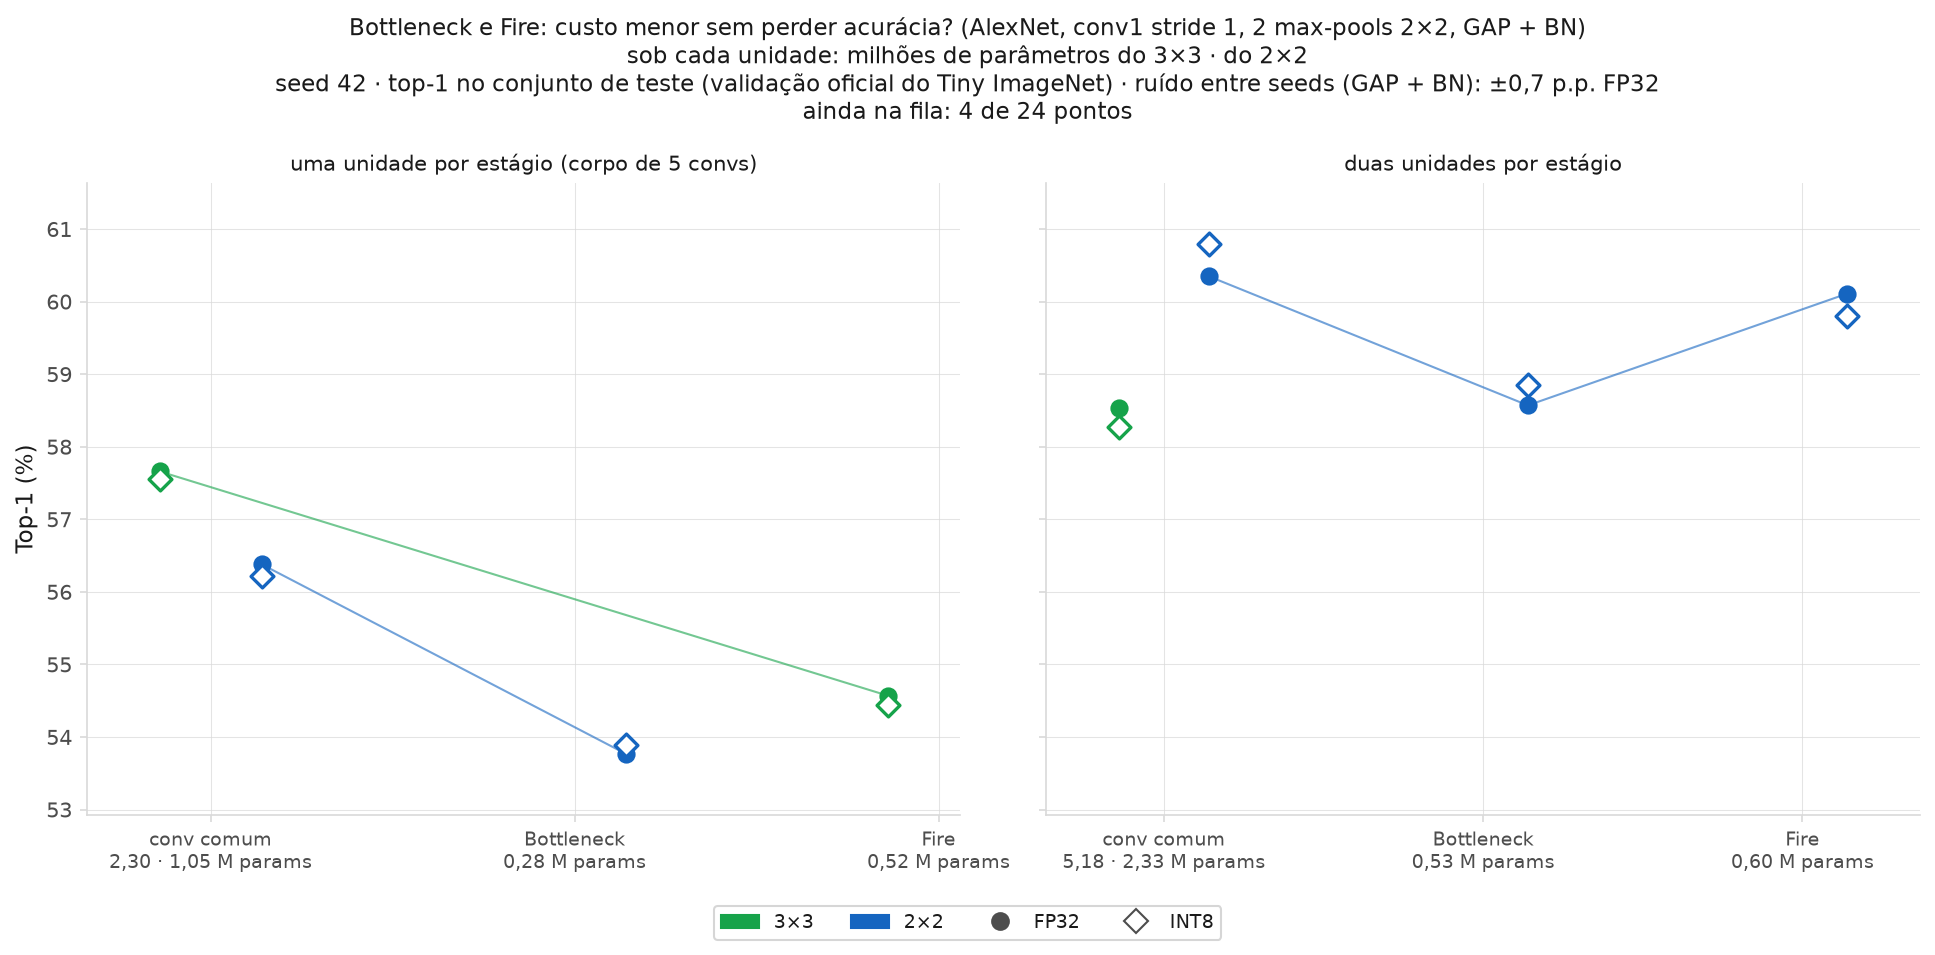
\includegraphics[width=\textwidth,trim=0 0 0 61.9,clip]{phase_13_bottleneck_fire/01_bottleneck_fire.png}
\caption{Blocos Bottleneck e Fire no corpo de stride 1 (AlexNet com GAP e BN, seed 42; variação de um treino: $\pm$0,7 p.p. em FP32). À esquerda, um bloco por estágio; à direita, dois. Círculo cheio: FP32; losango vazio: INT8; os pontos pequenos são as seeds 43 e 44, onde houver. Sob cada bloco estão os MACs do 3\by3 e, abaixo, os do 2\by2; entre parênteses, a parte que um acelerador Winograd executa (a regra da Tabela~\ref{tab:winograd}). A Fire 3\by3 com um bloco por estágio é a Fire do estudo principal.}
\label{fig:unidades}
\end{figure*}

Com um bloco por estágio, os blocos cortam de 70 a 83\% dos parâmetros e de 66 a 77\% dos MACs, mas perdem de 1,68 a 3,56 p.p. em FP32 nas quatro trocas, sempre além da variação de $\pm$0,7 p.p. Nesse caso, o Bottleneck fica à frente do Fire nos dois kernels (por 1,41 p.p. no 3\by3 e 0,95 p.p. no 2\by2).

Com dois blocos por estágio, a ordem se inverte: o Fire fica 1,27 p.p. (3\by3) e 1,54 p.p. (2\by2) acima do Bottleneck. No 2\by2, o Fire empata com o corpo comum ($-$0,24 p.p. na seed 42 e $-$0,68 p.p. na seed 43), com um quarto dos parâmetros e dos MACs. No 3\by3, ele fica 1,67 p.p. acima do corpo comum (60,20\% contra 58,53\%) e 1,50 p.p. acima da média de 3 seeds dele (58,70\%), com um quinto dos parâmetros e dos MACs. \pendente{Uma seed só: as seeds 43 e 44 desta rede estão na fila.} Com o Fire, os dois kernels ficam juntos (60,20\% e 60,11\%), enquanto os corpos comuns ficam 1,82 p.p. separados. Já o Bottleneck empata com o corpo comum no 3\by3 ($+$0,40 p.p.) e perde 1,78 p.p. no 2\by2.

Para um acelerador Winograd, o Fire é um meio-termo, porque os blocos põem parte da conta em convoluções 1\by1, que o acelerador não executa. Com dois por estágio, o Fire 3\by3 deixa no acelerador 76,9\% dos seus MACs, ou 283M, contra 1800M da rede comum, e põe 81M em convoluções 1\by1. O Fire 2\by2 deixa 59,7\%, e o Bottleneck, de 40 a 64\% nas quatro redes. O Fire reduz, portanto, o trabalho do acelerador em cerca de seis vezes sem perder acurácia, mas exige outra unidade para as convoluções 1\by1. É a mesma tensão da Seção~\ref{sec:hardware}, em escala menor.

\FloatBarrier

\subsection{Quanto a aritmética do acelerador Winograd custa em acurácia?}
\label{sec:numerica}

O custo depende do tamanho do bloco de saída (Figura~\ref{fig:numerica}). Os MACs das seções anteriores supõem uma conta exata, mas um acelerador
Winograd em FPGA faz a conta em ponto fixo, e o erro cresce com o bloco \cite{barabasz2020error}. Nas 16 redes simuladas, a mediana da diferença
para o FP32, no conjunto de teste, é de $-$0,2 p.p. em F(2,3) (de $-$0,7 a $+$3,8), $-$6,3 p.p. em F(4,3) (de $-$8,6 a $+$0,5) e $-$40,1 p.p. em F(6,3)
(de $-$59,8 a $-$10,5). Os valores mais altos de F(2,3) e F(4,3) são da AlexNet 3\by3 de layout original, cuja melhor época FP32 veio cedo: ali o QAT
também é treino extra (Seção~\ref{sec:int8}).

\begin{figure*}[!t]
\centering
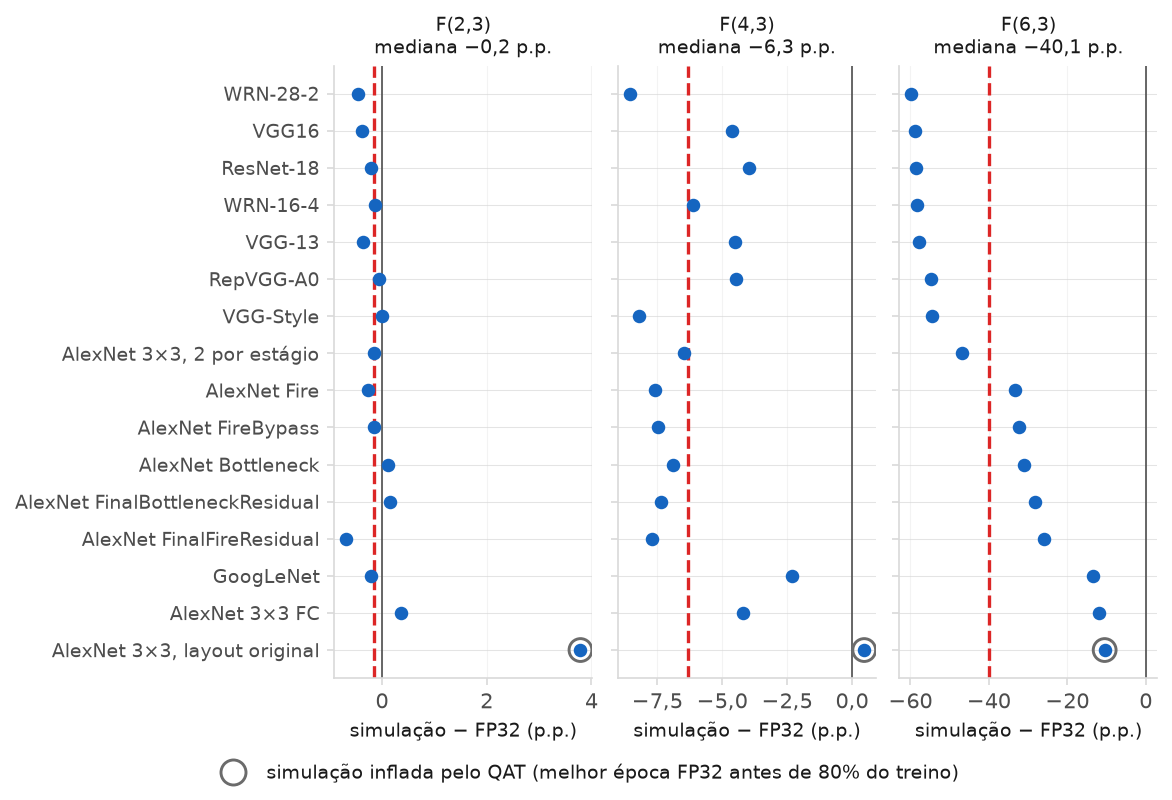
\includegraphics[width=0.86\textwidth]{phase_14_winograd_numerics/01_winograd_numerics.png}
\caption{Quanto a aritmética simulada do acelerador Winograd muda a acurácia de cada rede: simulação $-$ FP32 no conjunto de teste (uma seed por
rede), um painel por tamanho de bloco. A linha tracejada é a mediana das 16 redes; cada painel tem sua escala. O anel marca a rede cuja melhor
época FP32 veio cedo.}
\label{fig:numerica}
\end{figure*}

No F(6,3), porém, não se trata só de uma perda maior. Seis redes profundas (VGG-Style, VGG-13, VGG16, WRN-16-4, WRN-28-2 e ResNet-18) caem ao acaso, com 0,4 a
0,6\% de acerto, e a RepVGG-A0 fica em 4,2\%, enquanto as AlexNets ficam entre 11 e 28\%, e a GoogLeNet, em 48,5\%. Um estudo anterior do grupo, com outra
receita (AdamW, FP32 de até 100 épocas, 15 épocas de QAT medidas na validação), tinha achado $+$0,05, $-$5,1 e $-$18,9 p.p., e nele a mesma ResNet-18
chegava a 37,5\% em F(6,3).

A diferença entre os dois estudos não é falha de treino. Medimos a ResNet-18: cada camada F(6,3), sozinha, erra de forma parecida nas duas receitas (cosseno com a
convolução FP32 de 0,46 a 0,96 na nova e de 0,75 a 0,96 na anterior). O que muda é o acúmulo do erro, porque os observadores da quantização se calibram nas ativações da própria rede simulada, que já carregam o erro das camadas anteriores.
Na receita única, a partir da sétima convolução (13 de 19), eles ficam de 14 a 51 vezes acima do sinal limpo (de 1 a 3,7 vezes na anterior, em
todas). Nessas convoluções, só 2\% a 57\% das entradas diferentes de zero mantêm um código INT8 diferente de zero, e menos de 2\% dos blocos
transformados passam: quase nada chega ao fim da rede.

A VGG-13 colapsa do mesmo jeito: a partir da sexta convolução (5 de 10), os observadores
ficam de 12 a 34 vezes acima do sinal, e só 0,1\% a 2,4\% dos blocos passam. Já a GoogLeNet, com a mesma receita, não acumula o erro: os observadores
ficam no máximo 4,3 vezes acima do sinal, e pelo menos 29\% dos blocos passam em todas as convoluções. No início do QAT, as três estão no acaso em
F(6,3), mas só a GoogLeNet chega a 48,5\%. O que decide, portanto, é se o sinal atravessa a rede: sem sinal, o QAT não tem de onde partir. Não
medimos por que o erro se acumula em umas redes e não em outras.

\FloatBarrier

\section{Discussão}

\subsection{Como desenhar uma rede para Winograd}

Os resultados apontam para algumas escolhas:
\begin{itemize}
\item Acerte primeiro a geometria e o treino: use stride baixo na conv1 para imagens pequenas, BN e, na AlexNet, GAP. Esses fatores pesam tanto ou mais que o kernel. O stride 1 é o mais caro, pois quadruplica os MACs, e cabe a cada projeto decidir se vale esse custo.
\item Não aumente o kernel para ganhar acurácia: com GAP e BN, gastar a mais em largura ou em uma segunda convolução por estágio rende mais.
\item Use a conv1 11\by11 com cuidado. Ela ajuda um corpo de 5 convoluções, mas não acrescenta nada com dois por estágio e tira de 5 a 23 p.p. da parcela Winograd (10 p.p. no 2\by2 com dois por estágio).
\item Evite redes dominadas por convoluções \textit{depthwise} ou 1\by1 se o alvo é Winograd. Se a meta também é cortar custo, o Fire com dois blocos por estágio mantém a acurácia com um quarto a um quinto dos MACs e ainda deixa de 60 a 77\% deles no acelerador (Seção~\ref{sec:unidades}).
\item Não trate a quantização como obstáculo, mas confira se o FP32 convergiu antes do QAT, para não confundir treino extra com efeito da quantização.
\end{itemize}

\subsection{2\by2 ou 3\by3?}
\label{sec:2x2ou3x3}

A escolha depende do hardware. Em acurácia, com dois por estágio, o 2\by2 fica à frente e faz cerca de metade dos MACs diretos, ou cerca de 1,8 vez menos com Winograd (Seção~\ref{sec:hardware}). Esse kernel, porém, precisa de um acelerador preparado para ele.

A aritmética do acelerador também pesa (Seção~\ref{sec:numerica}). Os resultados de F($m$,3) vêm da simulação, não do hardware, e o kernel 2\by2
fica fora dessas transformações, então não há medida equivalente para F($m$,2). Assim, um acelerador com F(2,3) e redes 3\by3 é a opção sem custo de acurácia medido. Com F(4,3), a perda é de cerca de 6 p.p. (no pior caso, 8,6), e com F(6,3) o resultado depende da rede e, nas profundas, é inutilizável sem recalibrar as escalas.

\subsection{O que muda em relação ao trabalho anterior}

Sob a mesma receita, boa parte das diferenças entre redes de compensação desaparece. No relatório anterior \cite{souza2026relatorio}, um atalho residual em um bloco Fire \cite{iandola2016squeezenet} parecia ganhar mais de 6 p.p., mas os treinos seguiam protocolos diferentes, inclusive no número de épocas. Agora, Fire fica em 54,57\% e FireBypass em 55,19\%, uma diferença de 0,62 p.p., dentro da variação. As
redes Fire, FireBypass e as combinações com Fire e Bottleneck sem \textit{depthwise} ficam a menos de 1,5 p.p. umas das outras (de 54,40\% a 55,83\%, seed 42). O estudo de combinações aponta na mesma direção: o atalho não mostra ganho mensurável. Isso não invalida esses blocos, que continuam baratos, mas muda o motivo para usá-los.

As demais fases do projeto entram só como contexto, porque usaram protocolos diferentes. Medições anteriores em GPU indicaram que a aceleração Winograd depende de convoluções densas de stride 1. Em detecção, a compensação estrutural se transferiu só em parte. Em atenção local, o tamanho da janela se comportou como o tamanho do kernel \cite{souza2026relatorio}.

\subsection{Limitações}

A principal limitação é o número de seeds: a maioria das comparações usa uma só. As duas melhores redes só com 2\by2 foram repetidas com as seeds 43 e 44 e continuam acima da VGG16, mas as outras 22 combinações têm só a seed 42, entre elas a com conv1 11\by11 que empata com essas duas. Os blocos Bottleneck e Fire também têm só a seed 42, exceto o Fire 2\by2 com dois blocos por estágio, repetido com a seed 43.

O alcance da receita e dos controles também é limitado. A receita única não é a melhor para cada rede, e uma receita pode mudar a ordem entre arquiteturas \cite{bello2021revisiting,wightman2021resnet}; a taxa 0,02, por exemplo, pode melhorar as três redes testadas. O controle de capacidade e os testes de taxa e de CIFAR-100 usam GAP e BN, e o custo do 2\by2 com FC na AlexNet não foi explicado nem repetido. Os dados têm 64 px e 32 px, e as imagens de 224 px são apenas ampliações. Além disso, os três treinos da MobileNetV2 pré-treinada ficaram abaixo da nossa guarda de conversão, e a causa não foi investigada.

Do lado do hardware, nada foi medido em um acelerador real. Os resultados F($m$,3) têm uma seed por rede e vêm da simulação, e as escalas recalibradas, que poderiam evitar o colapso em F(6,3), não foram testadas. A parcela de MACs e a estimativa com Winograd usam só a geometria das camadas, e não medimos a vazão. Também não comparamos latência, porque os treinos rodaram em máquinas diferentes. Essa diferença faz parte da variação entre execuções e também afeta a seed 42 do estudo de combinações: as duas melhores redes foram treinadas em GPUs diferentes.

\section{Conclusão}

Restringir o kernel custa pouco quando o resto da rede está bem escolhido. Com GAP e BN, trocar os kernels originais da AlexNet por 3\by3 não custa nada, e a rede inteira em 2\by2 perde só 0,5 p.p. Nessa configuração, o custo do 2\by2 em relação ao 3\by3 vem da capacidade: com os mesmos MACs e parâmetros, os dois empatam. Com FC, porém, o custo na AlexNet chega a 6,5 p.p., e na VGG16 os dois empatam. Por isso, o custo do kernel
deve ser lido junto com o classificador e a família da rede.

A geometria e o BN costumam pesar mais que o kernel, e a quantização INT8 quase não pesa. Duas convoluções pequenas por estágio recuperam a perda e, nos pares testados, o 2\by2 fica à frente do 3\by3 com cerca de metade dos MACs. Com três seeds, essa vantagem de 1 a 2 p.p. se confirma sem atalho, mas não com atalho. Na aritmética do acelerador, o tamanho do bloco de saída custa mais acurácia do que a troca de kernel: F(2,3) quase não custa, e F(6,3) inutiliza a maioria das redes profundas. Com GAP e BN, o custo e a ordem dos kernels se repetem com outras taxas de aprendizado e no CIFAR-100.

Para quem projeta redes para aceleradores Winograd, a mensagem é simples: não é preciso manter kernels grandes no corpo da rede para ter boa acurácia, desde que a geometria e o classificador sejam escolhidos para isso.

\section{Trabalhos Futuros}

Queremos:
\begin{itemize}
\item fazer o controle de capacidade com classificador FC, para explicar o custo do 2\by2 na AlexNet;
\item reavaliar todas as redes no mesmo tipo de máquina, para comparar latência;
\item medir a vazão em um acelerador real;
\item investigar a MobileNetV2 pré-treinada em INT8;
\item repetir as comparações principais em imagens de resolução maior.
\end{itemize}

\section*{Agradecimentos}
Experimentos utilizaram recursos da infraestrutura PCAD (http://pcad.inf.ufrgs.br).

\renewcommand{\refname}{Referências}
\begin{thebibliography}{00}

\bibitem{lavin2016fast}
A. Lavin and S. Gray, ``Fast algorithms for convolutional neural networks,'' in \textit{Proc. IEEE Conf. Computer Vision and Pattern Recognition (CVPR)}, 2016.

\bibitem{barabasz2020error}
B. Barabasz, A. Anderson, K. M. Soodhalter, and D. Gregg, ``Error analysis and improving the accuracy of Winograd convolution for deep neural networks,'' \textit{ACM Transactions on Mathematical Software}, vol. 46, no. 4, Art. 37, 2020.

\bibitem{krizhevsky2012imagenet}
A. Krizhevsky, I. Sutskever, and G. E. Hinton, ``ImageNet classification with deep convolutional neural networks,'' in \textit{Advances in Neural Information Processing Systems (NeurIPS)}, 2012.

\bibitem{simonyan2015very}
K. Simonyan and A. Zisserman, ``Very deep convolutional networks for large-scale image recognition,'' in \textit{International Conference on Learning Representations (ICLR)}, 2015.

\bibitem{liu2022convnext}
Z. Liu, H. Mao, C.-Y. Wu, C. Feichtenhofer, T. Darrell, and S. Xie, ``A ConvNet for the 2020s,'' in \textit{Proc. IEEE/CVF Conf. Computer Vision and Pattern Recognition (CVPR)}, 2022.

\bibitem{ding2022scaling}
X. Ding, X. Zhang, Y. Zhou, J. Han, G. Ding, and J. Sun, ``Scaling up your kernels to 31x31: Revisiting large kernel design in CNNs,'' in \textit{Proc. IEEE/CVF Conf. Computer Vision and Pattern Recognition (CVPR)}, 2022.

\bibitem{souza2026relatorio}
R. S. de Souza and M. G. da Silva, ``Restrição do tamanho de kernel em CNNs para aceleração Winograd,'' relatório de pesquisa, Instituto de Informática, UFRGS, 2026.

\bibitem{bello2021revisiting}
I. Bello \textit{et al.}, ``Revisiting ResNets: Improved training and scaling strategies,'' in \textit{Advances in Neural Information Processing Systems (NeurIPS)}, 2021.

\bibitem{wightman2021resnet}
R. Wightman, H. Touvron, and H. Jégou, ``ResNet strikes back: An improved training procedure in timm,'' \textit{arXiv preprint arXiv:2110.00476}, 2021.

\bibitem{radosavovic2019network}
I. Radosavovic, J. Johnson, S. Xie, W.-Y. Lo, and P. Dollár, ``On network design spaces for visual recognition,'' in \textit{Proc. IEEE/CVF International Conference on Computer Vision (ICCV)}, 2019.

\bibitem{le2015tiny}
Y. Le and X. Yang, ``Tiny ImageNet visual recognition challenge,'' Stanford CS231N Report, 2015.

\bibitem{chrabaszcz2017downsampled}
P. Chrabaszcz, I. Loshchilov, and F. Hutter, ``A downsampled variant of ImageNet as an alternative to the CIFAR datasets,'' \textit{arXiv preprint arXiv:1707.08819}, 2017.

\bibitem{he2016deep}
K. He, X. Zhang, S. Ren, and J. Sun, ``Deep residual learning for image recognition,'' in \textit{Proc. IEEE Conf. Computer Vision and Pattern Recognition (CVPR)}, 2016.

\bibitem{cawley2010overfitting}
G. C. Cawley and N. L. C. Talbot, ``On over-fitting in model selection and subsequent selection bias in performance evaluation,'' \textit{Journal of Machine Learning Research}, vol. 11, 2010.

\bibitem{krizhevsky2009learning}
A. Krizhevsky, ``Learning multiple layers of features from tiny images,'' Technical Report, University of Toronto, 2009.

\bibitem{he2019bag}
T. He, Z. Zhang, H. Zhang, Z. Zhang, J. Xie, and M. Li, ``Bag of tricks for image classification with convolutional neural networks,'' in \textit{Proc. IEEE/CVF Conf. Computer Vision and Pattern Recognition (CVPR)}, 2019.

\bibitem{goyal2017accurate}
P. Goyal \textit{et al.}, ``Accurate, large minibatch SGD: Training ImageNet in 1 hour,'' \textit{arXiv preprint arXiv:1706.02677}, 2017.

\bibitem{szegedy2016rethinking}
C. Szegedy, V. Vanhoucke, S. Ioffe, J. Shlens, and Z. Wojna, ``Rethinking the Inception architecture for computer vision,'' in \textit{Proc. IEEE Conf. Computer Vision and Pattern Recognition (CVPR)}, 2016.

\bibitem{li2020budgeted}
M. Li, E. Yumer, and D. Ramanan, ``Budgeted training: Rethinking deep neural network training under resource constraints,'' in \textit{International Conference on Learning Representations (ICLR)}, 2020.

\bibitem{cubuk2019autoaugment}
E. D. Cubuk, B. Zoph, D. Mané, V. Vasudevan, and Q. V. Le, ``AutoAugment: Learning augmentation strategies from data,'' in \textit{Proc. IEEE Conf. Computer Vision and Pattern Recognition (CVPR)}, 2019, pp. 113--123.

\bibitem{he2015delving}
K. He, X. Zhang, S. Ren, and J. Sun, ``Delving deep into rectifiers: Surpassing human-level performance on ImageNet classification,'' in \textit{Proc. IEEE International Conference on Computer Vision (ICCV)}, 2015.

\bibitem{micikevicius2018mixed}
P. Micikevicius \textit{et al.}, ``Mixed precision training,'' in \textit{International Conference on Learning Representations (ICLR)}, 2018.

\bibitem{wu2019convolution}
S. Wu, G. Wang, P. Tang, F. Chen, and L. Shi, ``Convolution with even-sized kernels and symmetric padding,'' in \textit{Advances in Neural Information Processing Systems (NeurIPS)}, 2019.

\bibitem{jacob2018quantization}
B. Jacob \textit{et al.}, ``Quantization and training of neural networks for efficient integer-arithmetic-only inference,'' in \textit{Proc. IEEE Conf. Computer Vision and Pattern Recognition (CVPR)}, 2018.

\bibitem{wu2020integer}
H. Wu, P. Judd, X. Zhang, M. Isaev, and P. Micikevicius, ``Integer quantization for deep learning inference: Principles and empirical evaluation,'' \textit{arXiv preprint arXiv:2004.09602}, 2020.

\bibitem{nagel2021white}
M. Nagel, M. Fournarakis, R. A. Amjad, Y. Bondarenko, M. van Baalen, and T. Blankevoort, ``A white paper on neural network quantization,'' \textit{arXiv preprint arXiv:2106.08295}, 2021.

\bibitem{efron1993introduction}
B. Efron and R. J. Tibshirani, \textit{An Introduction to the Bootstrap}. Chapman \& Hall, 1993.

\bibitem{bouthillier2021accounting}
X. Bouthillier \textit{et al.}, ``Accounting for variance in machine learning benchmarks,'' in \textit{Proc. Machine Learning and Systems (MLSys)}, 2021.

\bibitem{luo2016understanding}
W. Luo, Y. Li, R. Urtasun, and R. Zemel, ``Understanding the effective receptive field in deep convolutional neural networks,'' in \textit{Advances in Neural Information Processing Systems (NeurIPS)}, 2016.

\bibitem{hooker2019what}
S. Hooker, A. Courville, G. Clark, Y. Dauphin, and A. Frome, ``What do compressed deep neural networks forget?'' \textit{arXiv preprint arXiv:1911.05248}, 2019.

\bibitem{kendall1938new}
M. G. Kendall, ``A new measure of rank correlation,'' \textit{Biometrika}, vol. 30, no. 1--2, pp. 81--93, 1938.

\bibitem{li2020rethinking}
H. Li \textit{et al.}, ``Rethinking the hyperparameters for fine-tuning,'' in \textit{International Conference on Learning Representations (ICLR)}, 2020.

\bibitem{iandola2016squeezenet}
F. N. Iandola, S. Han, M. W. Moskewicz, K. Ashraf, W. J. Dally, and K. Keutzer, ``SqueezeNet: AlexNet-level accuracy with 50x fewer parameters and $<$0.5MB model size,'' \textit{arXiv preprint arXiv:1602.07360}, 2016.

\end{thebibliography}

\appendix
\subsection{Figuras de apoio}
\label{sec:apendice}

As figuras a seguir trazem o detalhe por trás do texto: o efeito do stride da conv1, as imagens trocadas entre FP32 e INT8, a transferência para o CIFAR-100, a VGG16 com um kernel por bloco e as curvas de treino e de QAT, que mostram que as redes param de melhorar antes do fim das épocas.

\begin{figure*}[!t]
\centering
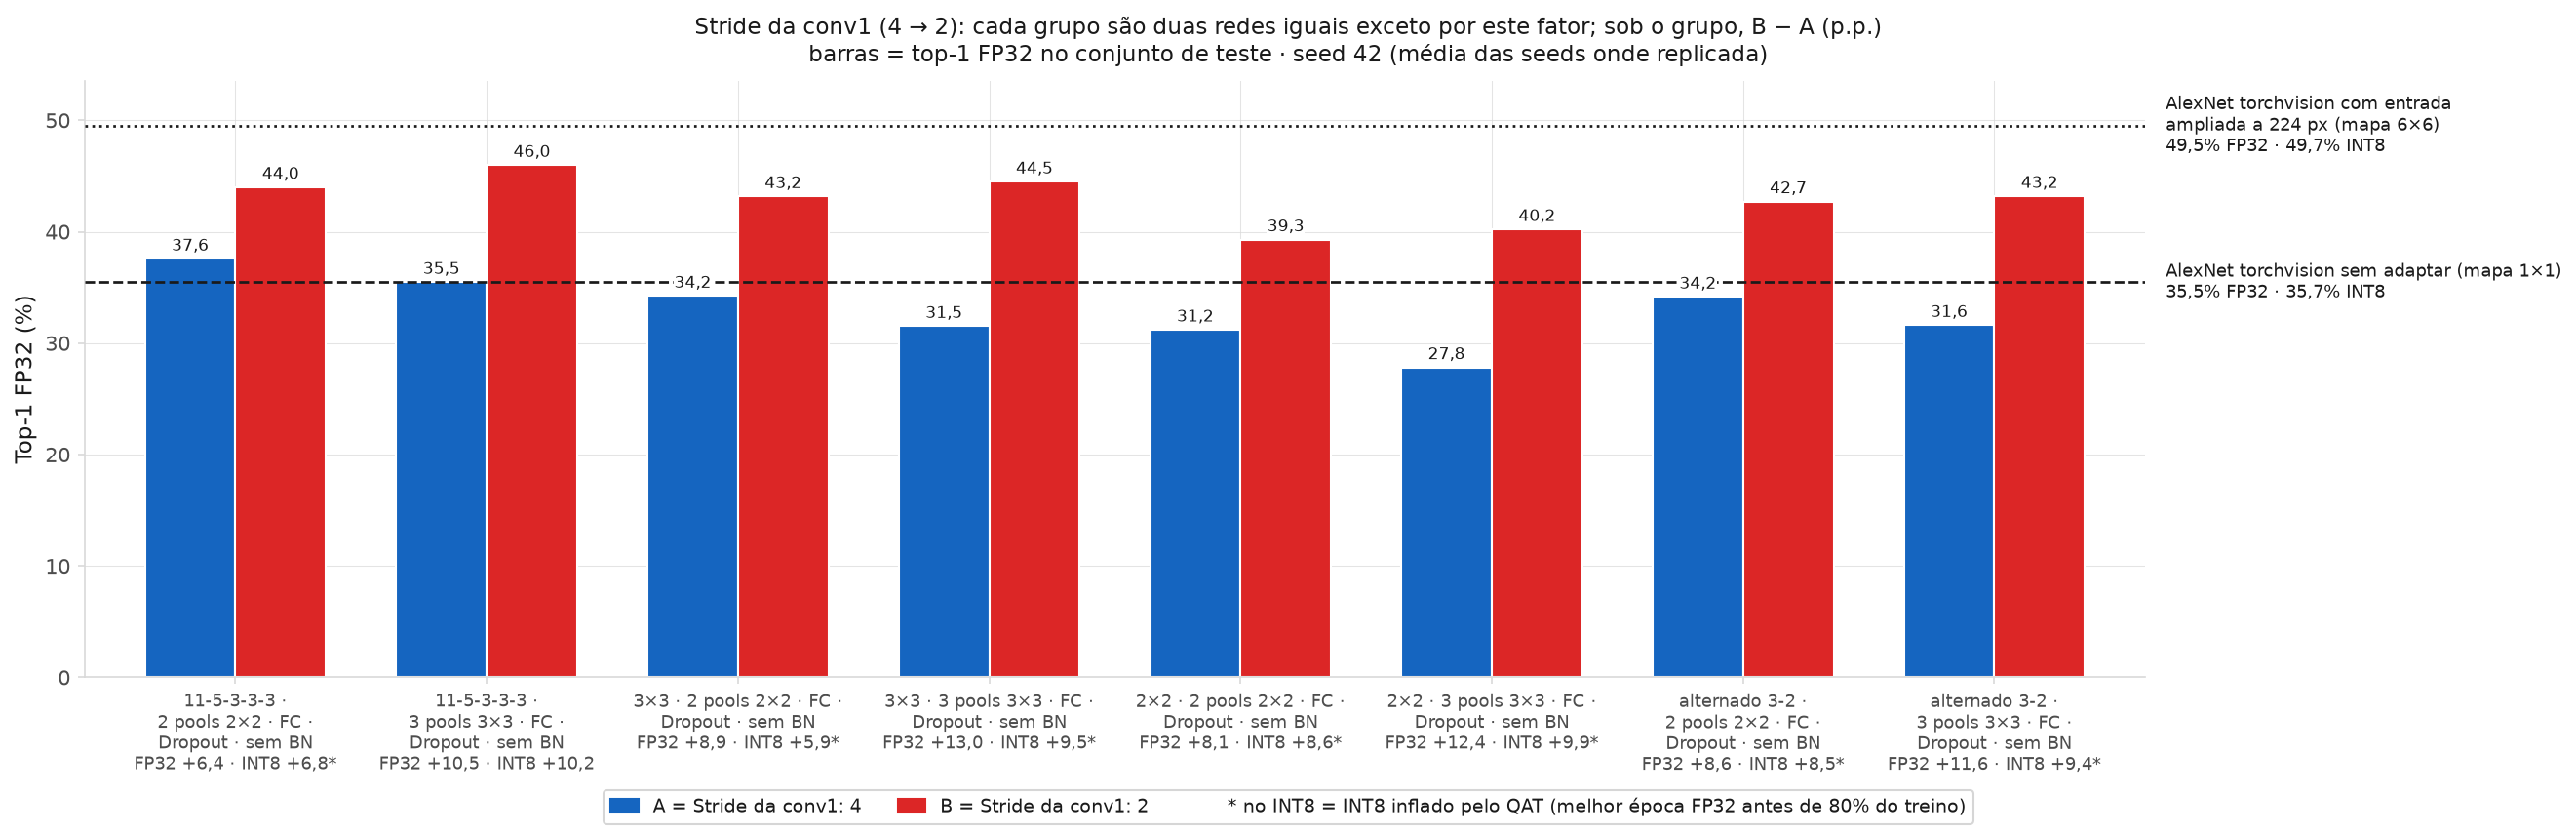
\includegraphics[width=\textwidth,trim=0 0 0 38.4,clip]{phase_11_kernel_size_comparison/05_conv1_stride.png}
\caption{O stride da conv1 pesa mais que o kernel. Em cada grupo, duas redes iguais exceto pelo stride: 4 (azul) ou 2 (vermelho). O stride 2 ganha nos oito pares. Barras: FP32 no teste, seed 42 (média das seeds onde houver). Sob cada grupo: B $-$ A em FP32 e em INT8 (asterisco: INT8 inflado pelo QAT). Linhas horizontais: a AlexNet sem adaptação e com a imagem ampliada para 224 px.}
\label{fig:stride}
\end{figure*}

\begin{figure*}[!t]
\centering
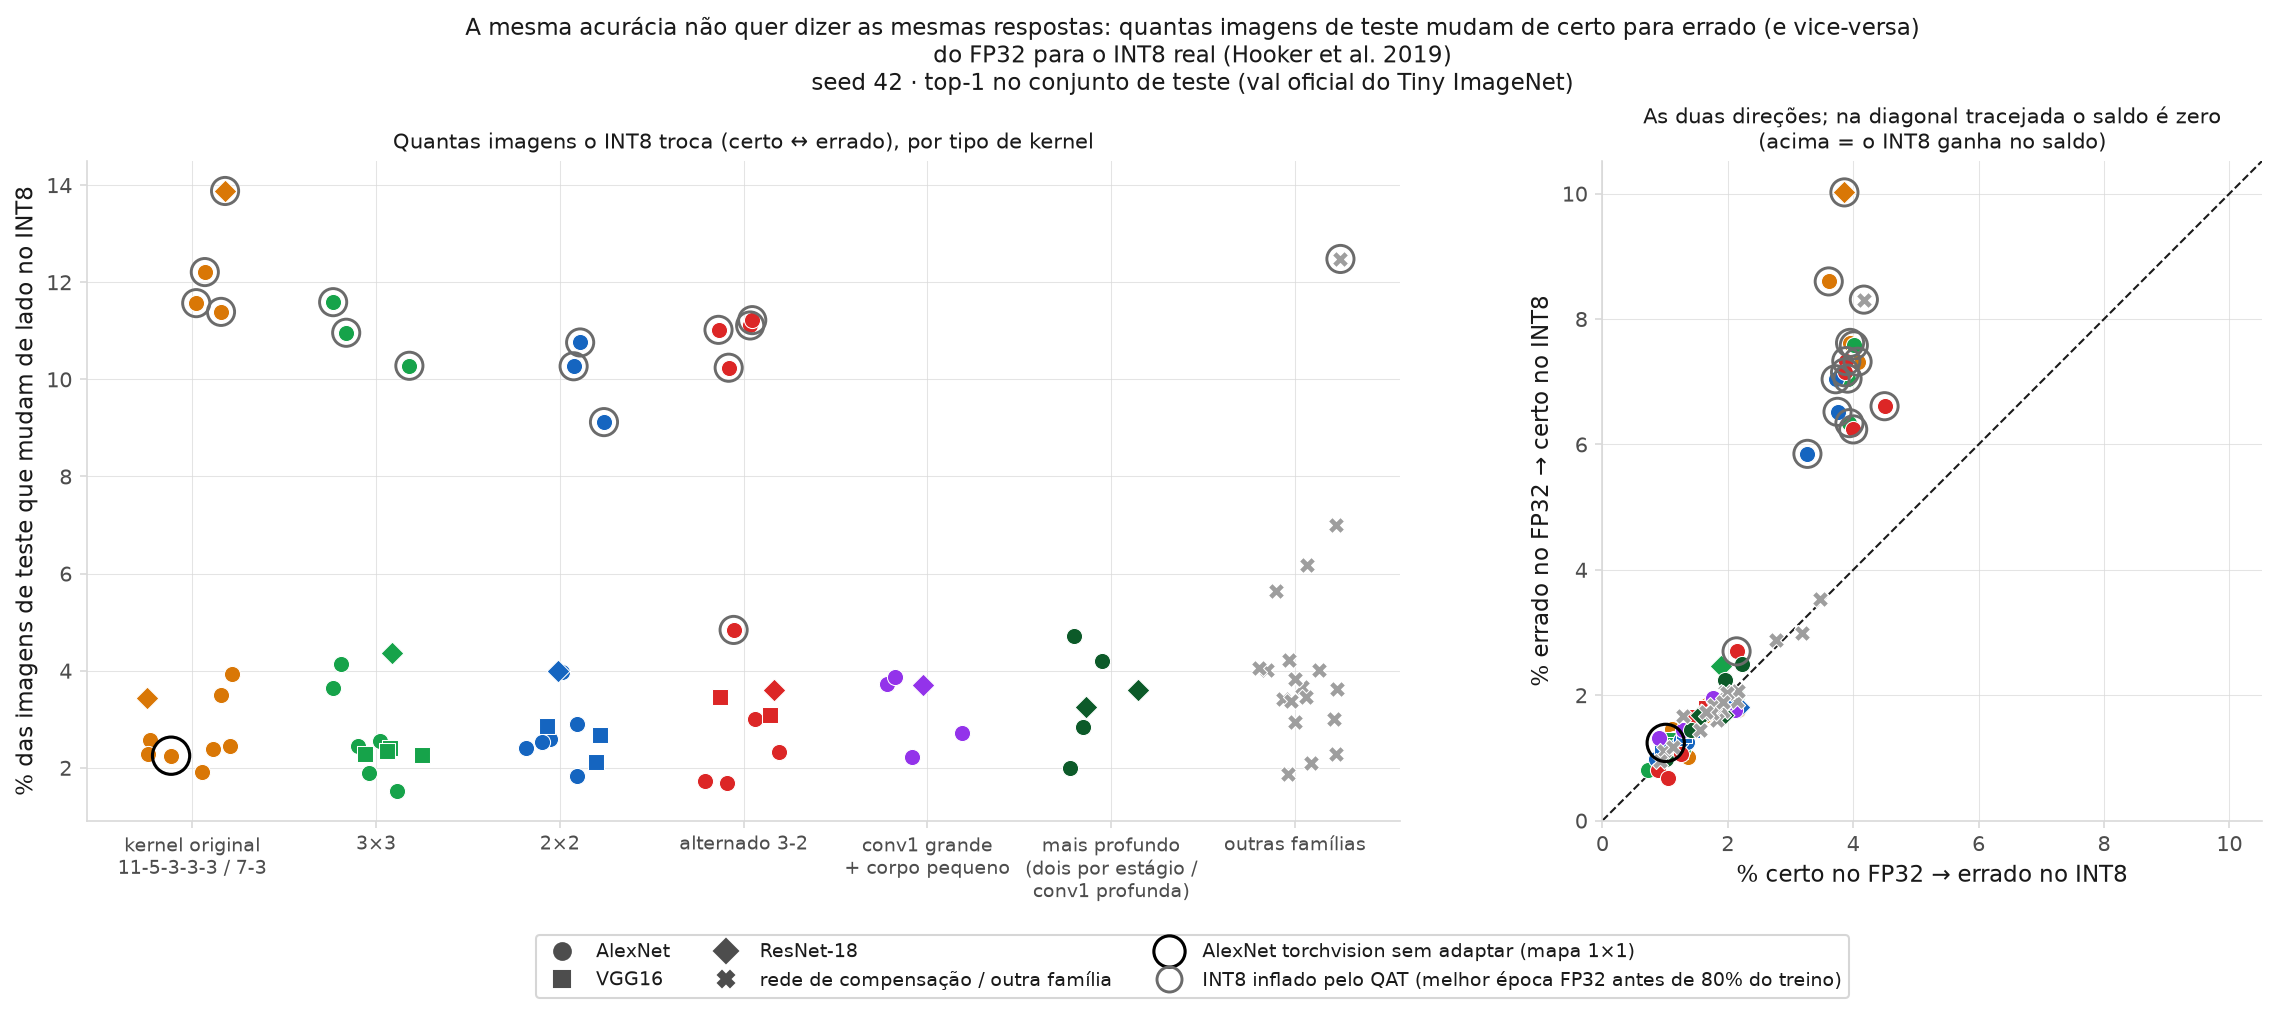
\includegraphics[width=\textwidth,trim=0 0 0 63.1,clip]{phase_11_kernel_size_comparison/20_int8_prediction_flips.png}
\caption{Imagens de teste que mudam entre certo e errado do FP32 para o INT8 (seed 42). À direita, sobre a diagonal, o saldo é zero. Só as redes com anel ficam claramente acima dela. O quadrado marca a AlexNet sem adaptação; os grupos são os da Figura~\ref{fig:int8}.}
\label{fig:flips}
\end{figure*}

\begin{figure*}[!t]
\centering
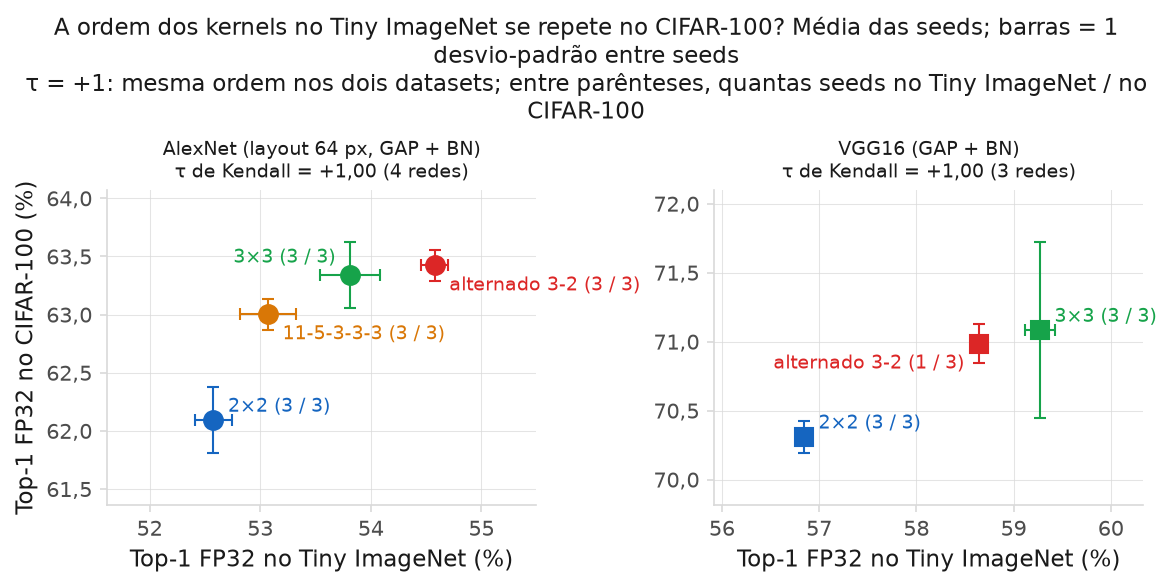
\includegraphics[width=0.86\textwidth,trim=0 0 0 62.4,clip]{phase_12_robustness/05_dataset_transfer.png}
\caption{A ordem dos kernels no Tiny ImageNet se repete no CIFAR-100, com GAP e BN. Cada ponto é a média das seeds, e as barras mostram um desvio-padrão entre seeds. Entre parênteses, quantas seeds no Tiny ImageNet e no CIFAR-100.}
\label{fig:transferencia}
\end{figure*}

\begin{figure*}[!t]
\centering
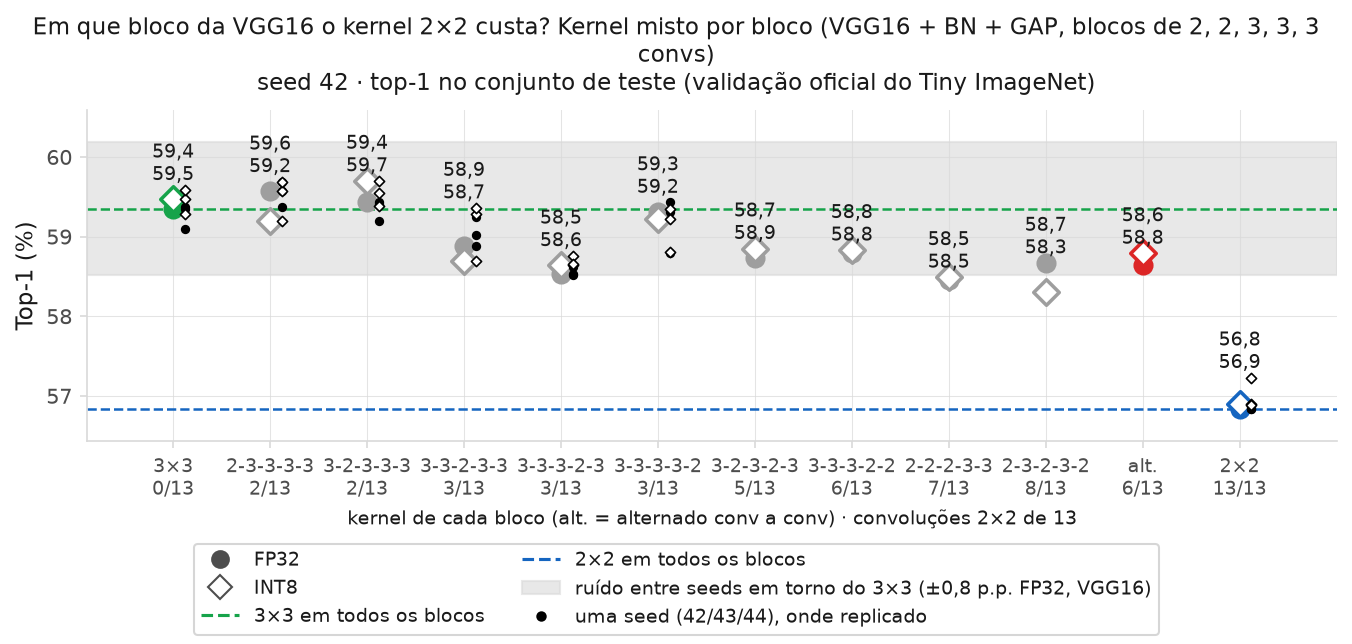
\includegraphics[width=\textwidth,trim=0 0 0 55.2,clip]{phase_11_kernel_size_comparison/24_vgg_kernel_blocks.png}
\caption{VGG16 com um kernel por bloco (GAP e BN; pontos: seed 42 e, onde houver, as outras seeds). Os padrões leem-se bloco a bloco: 3-3-3-2-3 tem 2\by2 só no bloco 4; abaixo, quantas das 13 convoluções são 2\by2. A faixa cinza é a variação de um treino em torno do 3\by3; a faixa para médias de 3 seeds é menor (Tabela~\ref{tab:ruido}).}
\label{fig:blocos}
\end{figure*}

\begin{figure*}[!t]
\centering
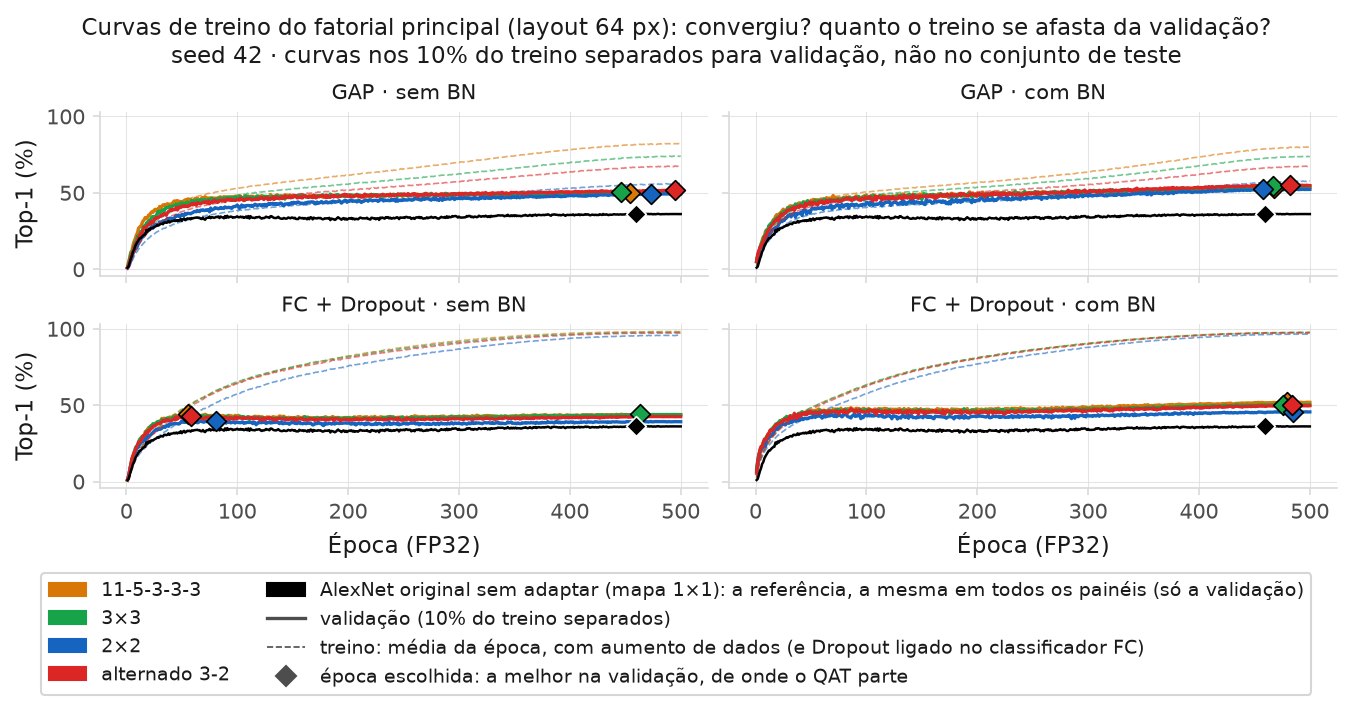
\includegraphics[width=\textwidth,trim=0 0 0 36.5,clip]{phase_11_kernel_size_comparison/18_training_curves.png}
\caption{Curvas de treino em FP32 (AlexNet de layout 64 px, seed 42), medidas nos 10\% do treino separados para validação. As redes com FC chegam perto de 100\% no treino, enquanto a validação fica parada. Nas redes com FC sem BN, a melhor época costuma vir cedo: são os casos marcados no texto.}
\label{fig:curvas_fp32}
\end{figure*}

\begin{figure*}[!t]
\centering
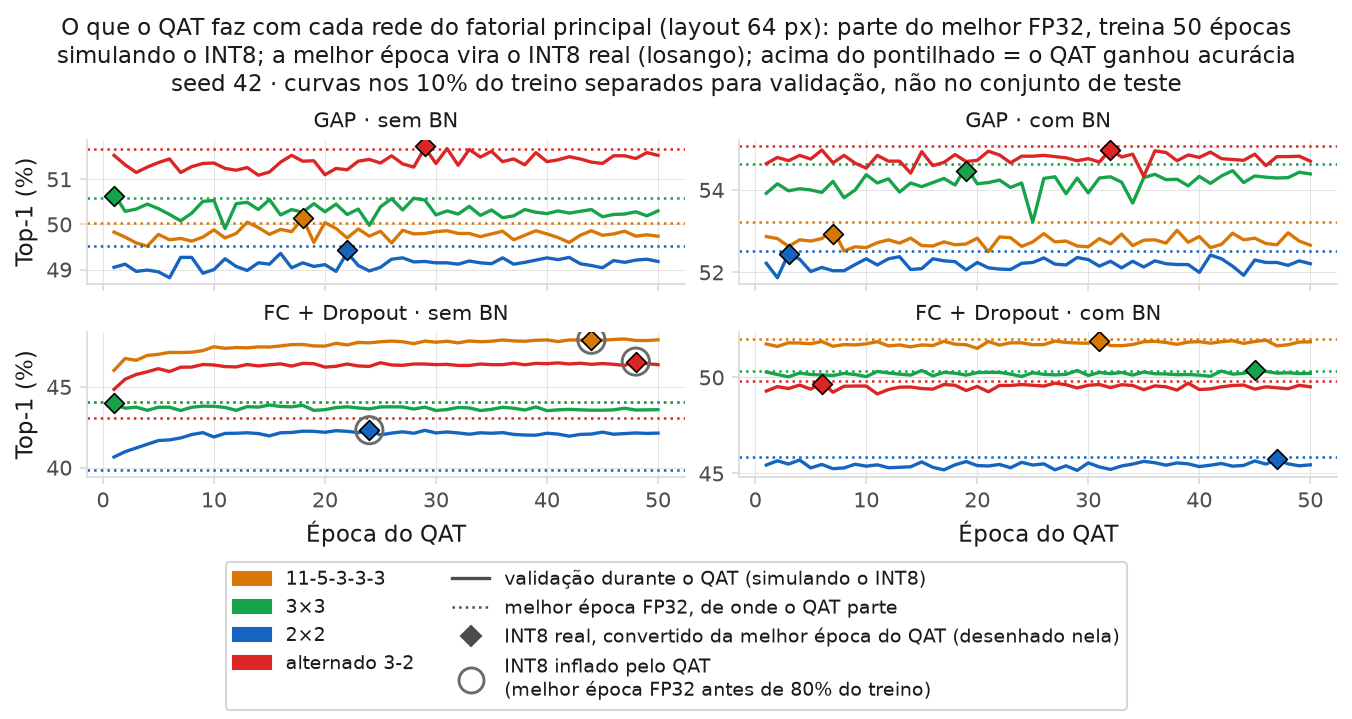
\includegraphics[width=\textwidth,trim=0 0 0 49.9,clip]{phase_11_kernel_size_comparison/19_qat_curves.png}
\caption{Curvas do QAT nas mesmas redes. O pontilhado é o FP32 de onde o QAT parte, e o losango é a época convertida para INT8. Só as redes com anel sobem claramente acima do ponto de partida: é o treino extra descrito na Seção~\ref{sec:int8}.}
\label{fig:curvas_qat}
\end{figure*}


\end{document}
